\chapter{Background Estimation}\label{chapter:bkg}
%Monte Carlo simulated samples are used to model the signal and background processes expected to be observed in the proton-proton collision data used.
%
%
%
%all the effects observed in 
%
%Typically, most of the discrepancies observed can be accounted for by applying various corrective scale factors.
%Where a particular process is poorly described and/or lacking sufficient statistics in the signal region, data-driven estimates of the background are used to model ...

\section{Data and Simulation Samples}\label{sec:samples}
Out of the 37.8\fbinv of  proton-proton collision data at $\sqrt{s} = 13\TeV$ collected by the CMS experiment during 2016, 35.8\fbinv was certified by the collaboration as being of sufficient quality to be used for physics analysis.
The difference between the certified value and the total data recorded is the result of various factors such as the unavailability of a detector due to power failures.
Due to the prescaling of all of the electron triggers considered during the start of the most luminous runs (as discussed in Section~\ref{sec:triggerStrategy}) the $ee$ channel uses a reduced dataset corresponding to 35.6\fbinv where none of the triggers considered were prescaled.

The MC samples used to model both the model signal and background processes considered here are listed in table~\ref{tab:mcList}.
For each of the processes considered, the table which includes information on the number of events generated, the cross section used in their generation and the order in perturbative accuracy in QCD to which the generators calculated the processes.
For all the MC samples considered, the hadronisation performed was undertaken using PYTHIA 8 which used the CUETP8M2T4 underlying event tune.
The NNPDF3.0 family of PDF sets~\cite{Ball:2012cx} was used as for sample generation, where the exact set chosen depended on whether the sample was produced at LO or NLO and used either the four or five flavour scheme.

\begin{table}[htbp]
\topcaption {
The MC processes and their associated sample sizes, cross sections and generators used. Two generators are considered for the simulation of the Z+jets process; both samples are included in the table.
}
\label{tab:mcList}
  \centering
  \resizebox{\textwidth}{!}{
% This right-aligns numbers in column, but centers them under column title.
 \begin{tabular}{cccc}
   \hline
   \textbf{MC process} & \textbf{Events} & \textbf{Cross section (pb)} & \textbf{Generator (Order)}   \\
   \hline
   tZq  & 14.5M & 0.0758  & aMC@NLO (NLO) \\
   \hline
   tHq  & 3.5M & 0.07462  & Madgraph (LO) \\
   \hline
   tWZ/tWll  & 50K & 0.01104  & Madgraph (LO) \\
   \hline
   t tW-channel & 7M & 35.85 & POWHEG (NLO) \\
   $\overline{\text{t}}$ tW-channel & 6.9M & 35.85 & POWHEG (NLO) \\
   \hline
   t s-channel & 2.9M & 10.32 & aMC@NLO (NLO) \\
   \hline
   t t-channel & 67.2M & 136.02 & POWHEG (NLO) \\
   $\overline{\text{t}}$ t-channel & 38.8M & 80.95 & POWHEG (NLO) \\
   \hline
   \ttbar & 77.1M & 831.76 & POWHEG (NLO) \\
   \hline
   \ttbarZ $\rightarrow$ ll$\nu\nu$ & 13.9M & 0.2529   & aMC@NLO (NLO) \\
   \ttbarZ $\rightarrow$ qq & 749K & 0.5297   & aMC@NLO (NLO) \\
   \hline
   \ttbarW $\rightarrow$ l$\nu$ & 5.3M & 0.2001   & aMC@NLO (NLO) \\
   \ttbarW $\rightarrow$ qq & 833K & 0.405  & aMC@NLO (NLO) \\
   \hline
   \ttbarH $\rightarrow$ bb & 3.8M & 0.2942 & POWHEG (NLO) \\
           $\rightarrow$ non bb & 4.0M & 0.2123 & POWHEG (NLO) \\
   \hline
   W+jets & 24.1M & 61526.7 & aMC@NLO (NLO) \\
   \hline
   Z+jets ($m_{Z} \geq 50\GeVcc $) & 146M & 5765.4 & Madgraph (LO) \\
   Z+jets ($10 \GeVcc \leq m_{Z} < 50\GeVcc$) & 35.3M & 18610.0 & Madgraph (LO) \\
   \hline
   Z+jets ($m_{Z} \geq 50\GeVcc $) & 151M & 5765.4 & aMC@NLO (NLO) \\
   Z+jets ($10 \GeVcc \leq m_{Z} < 50\GeVcc$) & 106M & 18610.0 & aMC@NLO (NLO) \\
   \hline
   WW $\rightarrow$ l$\nu$qq & 9.0M & 49.997  & POWHEG (NLO) \\
      $\rightarrow$ ll$nu\nu$ & 2.0M & 12.178 & POWHEG (NLO) \\
   \hline
   WZ $\rightarrow$ l$\nu$qq & 24.2M & 10.73 & aMC@NLO (NLO) \\
      $\rightarrow$ llqq & 26.5M & 5.606 & aMC@NLO (NLO) \\
      $\rightarrow$ lll$\nu$ & 1.9M & 5.26 & aMC@NLO (NLO) \\
   \hline
   ZZ $\rightarrow$ ll$\nu\nu$ & 8.8M & 0.5644 & POWHEG (NLO) \\
      $\rightarrow$ llqq & 15.3M & 3.222 & aMC@NLO (NLO) \\
      $\rightarrow$ llll & 10.7M & 1.204 & aMC@NLO (NLO) \\
   \hline
   WWW & 240K & 0.2086 & aMC@NLO (NLO) \\
   \hline
   WWZ & 250K & 0.1651 & aMC@NLO (NLO) \\
   \hline
   WZZ & 247K & 0.05565 & aMC@NLO (NLO) \\
   \hline
   ZZZ & 249K & 0.01398 & aMC@NLO (NLO) \\
   \hline
   
 \end{tabular}}
\end{table}

To determine the impact of a variety of different theoretical uncertainties for several of the processes defined in table~\ref{tab:mcList}, dedicated MC samples were used, which are listed in table~\ref{tab:theorySampleList}.
The entries labelled ``scale'' denote samples where the renormalisation and factorisation scales for PS has been varied ``up'' by a factor of 2 and ``down'' by a factor of 0.5.
For \ttbar simulation samples, the initial state radiation (ISR) and final state radiation (FSR) scales are varied independently, with corresponding samples in the table.
The entries labelled ``matching'' denote samples where the energy threshold used in the ME/PS matching is varied.
These uncertainties are discussed further in Section~\ref{sec:theorySysts}.

\begin{table}[htbp]
\topcaption {
The dedicated MC samples used to estimate some theoretical uncertainties. The table includes the associated size of the samples, cross sections and generators used.
}
\label{tab:theorySampleList}
  \centering
 \resizebox{\textwidth}{!}{
 \begin{tabular}{cccc}
   \hline
   \textbf{MC process} & \textbf{Events} & \textbf{Cross section (pb)} & \textbf{Generator (Order)}   \\
   \hline
   tZq scale up & 6.9M & 0.0758  & aMC@NLO (NLO) \\
   tZq scale down & 7.0M & 0.0758  & aMC@NLO (NLO) \\
   \hline
   t tW-channel scale up & 998K & 35.85 & POWHEG (NLO) \\
   t tW-channel scale down & 994K & 35.85 & POWHEG (NLO) \\
   $\overline{\text{t}}$ tW-channel scale down & 1.0M & 35.85 & POWHEG (NLO) \\
   $\overline{\text{t}}$ tW-channel scale down & 999K & 35.85 & POWHEG (NLO) \\
   \hline
   t t-channel scale up & 5.7M & 136.02 & POWHEG (NLO) \\
   t t-channel scale down & 5.9M & 136.02 & POWHEG (NLO) \\
   t t-channel matching up & 6.0M & 136.02 & POWHEG (NLO) \\
   t t-channel matching down & 6.0M & 136.02 & POWHEG (NLO) \\
   $\overline{\text{t}}$ t-channel scale up & 4.0M & 80.95 & POWHEG (NLO) \\
   $\overline{\text{t}}$ t-channel scale down & 3.9M & 80.95 & POWHEG (NLO) \\
   $\overline{\text{t}}$ t-channel matching up & 4.0M & 80.95 & POWHEG (NLO) \\
   $\overline{\text{t}}$ t-channel matching down & 4.0M & 80.95 & POWHEG (NLO) \\
   \hline
   \ttbar ISR up & 156.5M & 831.76 & POWHEG (NLO) \\
   \ttbar ISR down & 149.8M & 831.76 & POWHEG (NLO) \\
   \ttbar FSR up & 152.6M & 831.76 & POWHEG (NLO) \\
   \ttbar FSR down & 156.0M & 831.76 & POWHEG (NLO) \\
   \ttbar matching up & 58.9M & 831.76 & POWHEG (NLO) \\
   \ttbar matching down & 58.2M & 831.76 & POWHEG (NLO) \\
   \hline   
 \end{tabular}}
\end{table}

%%% Alt Z+jets 
%During the study of the poor agreement between simulation and data for the aMC@NLO Z+jets samples considered, a number of alternative 
%To determine the impact of a number of theoretical uncertainties for a number of processes, a several dedicated samples, listed in table~\ref{tab:zPlusSamples}, were used.
%These systematic uncertainties are discussed further Section~\ref{sec:subsec:zPlusJetsEstimation}.
%
%\begin{table}[htbp]
%\topcaption {
%The dedicated MC samples used to determine the impact of theoretical uncertainties, including the associated total number of events, cross sections and generators (and order in perturbative QCD accuracy they are calculated to), considered for the search for tZq in the dilepton final state.
%}
%\label{tab:zPlusSamples}
%  \centering
% \resizebox{\textwidth}{!}{
% \begin{tabular}{cccc}
%   \hline
%   \textbf{MC process} & \textbf{Events} & \textbf{Cross section (pb)} & \textbf{Generator (Order)}   \\
%   \hline
%   tZq scale up & 6.9M & 0.0758  & aMC@NLO (NLO) \\
%   \hline   
% \end{tabular}}
%\end{table}
%

\section{Simulation Corrections}\label{sec:simCorrections}
Simulation is unable to fully recreate all the effects observed in data corrective scale factors are used to reweight MC samples on a per event basis to account for possible discrepancies.

These scale factors are used to correct the simulation for any discrepencies in the lepton identification, isolation and reconstruction efficiencies, lepton and jet energy scales and resolutions, b-tagging efficiencies, the poor modelling of pileup in simulation, and the detector resolutions observed in data.

\subsection{Miscalibrated Tracker APV}\label{subsec:hipEffect}
During the first half of data taking in 2016 the silicon strip detector suffered from an instantaneous-luminosity-dependent hit finding inefficiency, which particularly affected high occupancy regions, due to saturation in the pre-amplifier in the front-end electronics~\cite{Fiori:2016ebh}.
This issue was resolved by changing the configuration of the electronics.
The 55\% of the total dataset affected by this issue has since been reprocessed by CMS to mitigate the impact on the quality of the data taken.

Despite this however, there is still a negative impact on the reconstructing tracks efficiency for physics objects that rely upon tracking data.

This reduced detector efficiency is accounted for by using the weighted average of the scale factors that have been derived separately for both the affected and unaffected portions of the dataset.

\subsection{Lepton Efficiency}\label{subsec:leptonRecoSFs}
The identification, isolation and reconstruction efficiency scale factors for leptons are produced centrally by CMS and are determined by using a large sample of of $Z \rightarrow l^{+} l ^{-}$ events and the so-called \emph{tag-and-probe} method~\cite{CMS:2008rxa}.
From a high-purity sub-sample of these events, where the dilepton invariant mass lies within the window $60 < m_{ll} < 120 \GeV$, the lepton that passes a tight selection criteria is ``tagged'' and other lepton is ``probed'' against a loose selection criteria.
For each type and lepton flavour, the efficiency is the fraction of events where the probe leptons passed the selection criteria under study.
The corrective scale factors determined from these efficiencies are used to reweight events as functions of their leptons' \pt, $\eta$, and flavour.

The triggers efficiencies for the analysis were determined by the author by using events that pass other trigger combinations that are weakly correlated with those used in the analysis, known as \emph{cross triggers} (X triggers).
The trigger efficiency is estimated as follows:

\begin{equation}
\epsilon_{trigger} = \frac{N_{X triggers + lepton triggers}}{N_{X triggers}} \;
\end{equation}

where $N_{X trigger}$ is the number of events that have passed the analysis' lepton selection criteria and the cross triggers, and $N_{X triggers + lepton triggers}$ is $N_{X trigger}$ and the number of events that additionally passed at least one of the lepton triggers for the relevant lepton flavour.

As the trigger requirements are applied to both simulated and data events, a scale factor of the ratio of the trigger efficiency in data and in simulation is calculations and used to weight the simulation.
For both the $ee$ and $\mu\mu$ channels in the signal region and the $e \mu$ channel for the \ttbar control region, a constant scale factor was found to be sufficient to account for the differences between data and simulation.

The efficiencies were determined using data and simulated \ttbar events.
The resultant trigger efficiency scale factors applied to simulation are given in table~\ref{tab:triggerSFs} with their associated statistical uncertainties.
The associated systematic uncertainties are discussed in Section~\ref{sec:systematics}.

\begin{table}[htbp]
\topcaption {The trigger efficiencies for the lepton selection criteria for data and simulation and the resultant corrective scale factors applied to simulation. The uncertainties given only include the statistical uncertainty associated with each value. The determination of the systematic uncertainties is given in Section~\ref{sec:systematics}.}
\label{tab:triggerSFs}
  \centering
  \resizebox{\textwidth}{!}{
 This right-aligns numbers in column, but centers them under column title.
 \begin{tabular}{lccc}
   \hline
   \textbf{Channel} & \textbf{$\epsilon _{data}$} & \textbf{$\epsilon _{MC}$} & \textbf{Scale Factor}\\
   \hline   
   $ee$ & 0.976 $\pm$ 0.001 & 0.988 $\pm$ 0.001 & 0.987 $\pm$ 0.001\\
   $\mu\mu$ & 0.985 $\pm$ 0.001 & 0.992 $\pm$ 0.001 & 0.993 $\pm$ 0.000  \\
   $e \mu$ & 0.875 $\pm$ 0.014 & 0.882 $\pm$ 0.019 & 0.991 $\pm$ 0.007\\
   \hline
 \end{tabular}}
\end{table}

% part 1 mumu
%% data eff 0.98069  +/- -0.00070/0.00073
%% SF 0.98868 +/- 0.00013
 part 2 mumu
%% data eff 0.99061 +/- -0.00057/0.00061
%% MC 0.99192 +/- -0.00061/0.00074
%% SF 0.99868 +/- 0.00017

%%  lumiRunsBCDEF_{19713.888}, // Lumi for hip era runs
%  lumiRunsGH_{16146.178}, // Lumi for post-hip era runs

\subsection{Lepton Energy Corrections}\label{subsec:leptonEnergyCorrections}
\subsubsection{Electron Regression and Energy Scale and Smearing Corrections}
Energy regression and energy scale and smearing corrections that have been produced by the CMS Electron Gamma (EGM) Physics Object Group.
The energy regression uses detector information to correct the electron energy recorded in order to obtain the best possible resolution of the reconstructed particle.
The energy scale and smearing corrections are used to correct the energy scale and resolution in simulation.

\subsubsection{Rochester Corrections}
The muon momentum scale and resolution correction methods developed by the University of Rochester~\cite{rochester}, known as \emph{Rochester Corrections}, are used to remove any muon momentum bias arising from any possible detector misalignment and any error in the measurement of the magnetic field for both MC and data.
These corrections are derived using a sample of high \pt $> 20\GeVc$ muons from Z $ \rightarrow \mu^{+}\mu^{-}$ decays using a two-step method.
The first of the two steps determines a correction factor that is defined as the difference in the mean inverse transverse momenta of the muons from a perfectly aligned simulation and reconstructed data or simulation.
These corrections are tuned in the second step using the $M_{\mu^mu}$ peak for a perfectly aligned detector to calibrate the corrections.
This removes any dependence on detector efficiency or physics modelling.

The Rochester Corrections are applied to each muon as an event weight that is a function of the muon's charge, \pt, $\eta$ and $\phi$.

\subsection{Jet Energy Corrections}\label{subsec:jesjer}
As described in Section~\ref{subsubsec:JECs}, the Jet Energy Corrections are applied to account for the non-uniform response in \pT and $\eta$ of the detector by comparing the differences between the generator level and detector level responses in simulation and any residual differences between simulation and data.

In addition to these corrections, as the Jet Energy Resolution (JER) observed in data is approximately 10\% poorer than that observed in simulation, the 4-vectors of simulated jets are smeared as functions of generator level and reconstructed \pt and $\eta$ to account for this~\cite{Khachatryan:2016kdb}.

\subsection{b-tagging Efficiency}\label{subsec:btagEff}
The CMS B-Tag and Vertexing (BTV) Physics Object Group measures the b-tagging efficiency and misidentification rates for b- and light-flavoured jets in data and MC simulation considering both multijet and \ttbar processes for the algorithms that they support~\cite{Sirunyan:2017ezt}.
From these measurements b-tagging efficiency scale factors are produced and provided for analysts to apply to simulated events to correct for differences observed between data and simulation.
These scale factors, as functions of the jet flavour, \pT and $\eta$, are used to alter the weight of the MC events.
This methodology was chosen as it involves only changing the weight of the selected MC events which, unlike other methods, avoids events migrating into different b-tag multiplicity bins and having events with potentially undefined variables such as the top mass.

\subsection{\PU Modelling}\label{subsec:puSF}
It is challenging to model variations in the number of \PU interactions that result from the changing LHC conditions.
To achieve this, MC events are reweighted as a function of the number of primary vertices so that the simulated PU distributions resemble those observed in data.

The \PU SF is determined as a function of the number of primary vertices, $n_{PV}$, by comparing the $n_{PV}$ distribution in minimum bias data over the running period considered to the corresponding $n_{PV}$ distribution in simulated events.

\subsection{Top quark \pt}
A scale factor is used to reweight all simulated \ttbar events to account for the differences in the top quark \pt distribution observed between data and both the LO and NLO MC simulation~\cite{Khachatryan:2015oqa}.

%\section{Signal Region Simulated Backgrounds}\label{sec:simBackgrounds}
A comparison between data and simulation, after all corrections have been applied, in the signal region 

While the jet cleaning and tight isolation criteria for leptons has significantly reduced the non-prompt lepton contributions and reduced contributions from the W+jets process to negligible levels, the signal region is still dominated by a number of background processes.
The two most dominant background processes are Z+jets and \ttbar production, with contributions of a similar size to that from the tZq process from the tW, \ttbarZ, WZ and ZZ processes.
The remaining single top (tHq, tWZ, s-channel, t-channel), \ttbarW, \ttbarH, WW and triboson backgrounds produce contributions smaller than the signal process.

\section{Signal Region Background Estimation}
A comparison between data and simulation (after all corrections have been applied) is shown in 

\begin{table}[htbp]
\topcaption{The number of observed events in data, the data-driven estimate of the non-prompt leptons and the number of expected events in simulation in the signal region following the full event selection for each of the separate channels and with both channels combined. The aMC@NLO sample is used for the Z+jets contribution.
}\label{tab:signalYields}
\centering
\begin{tabular}{lccc}
\hline
Channel &  $ee$ & $\mu\mu$ & Combined \\
\hline
Signal (SM tZq) & 30.38$\pm$0.04 & 55.49 $\pm$ 0.07 & 85.87 $\pm$ 0.11 \\
Backgrounds: & & & \\
tWZ\@: & 6.38$\pm$0.13 & 10.96$\pm$0.23 & 17.34$\pm$0.36    \\
tHq: & 0.17$\pm$0.01 & 0.37$\pm$0.01 & 0.54$\pm$0.02    \\
ttW\@: & 7.38$\pm$0.08 & 10.83$\pm$0.12 & 18.21$\pm$0.20    \\
ttZ\@: & 62.23$\pm$0.13 & 111.98$\pm$0.23 & 174.21$\pm$0.36    \\
ttH\@: & 4.94$\pm$0.06 & 9.73$\pm$0.11 & 14.67$\pm$0.17    \\
\ttbar: & 1658.73$\pm$14.00 & 3277.48$\pm$27.66 & 4936.21$\pm$41.66    \\
tW\@: & 55.98$\pm$2.52 & 109.59$\pm$4.49 & 165.57$\pm$7.01    \\
s-channel: & 0.0 $\pm$ 0.0 & 0.19$\pm$0.19 & 0.19$\pm$0.19    \\
t-channel: & 0.61$\pm$0.14 & 1.12$\pm$0.31 & 1.73$\pm$0.45    \\
WW\@: & 1.34$\pm$0.31 & 2.29$\pm$0.52 & 3.63$\pm$0.83    \\
WZ\@: & 72.88$\pm$0.41 & 127.32$\pm$0.71 & 200.20$\pm$1.12    \\
ZZ\@: & 51.80$\pm$0.30 & 94.64$\pm$0.55 & 146.44$\pm$0.85    \\
WWW\@: & 0.11$\pm$0.03 & 0.27$\pm$0.08 & 0.38$\pm$0.11    \\
WWZ\@: & 1.32$\pm$0.10 & 2.20$\pm$0.17 & 3.32$\pm$0.27    \\
WZZ\@: & 1.53$\pm$0.07 & 2.62$\pm$0.11 & 4.15$\pm$0.18    \\
ZZZ\@: & 0.65$\pm$0.02 & 1.12$\pm$0.04 & 1.77$\pm$0.06    \\
W + jets: & 0.0$\pm$0.0 & 0.0$\pm$0.0 & 0.0$\pm$0.0    \\
Z + jets: & 3290.64$\pm$27.53 & 5877.51$\pm$87.78 & 9168.15$\pm$115.31    \\
\hline
NPLs: & 69.47$\pm$0.76 & 114.01$\pm$1.25 & 183.48$\pm$2.01   \\
\hline
Data & 5274.0$\pm$72.62 & 9750.0$\pm$98.74 & 15024.0$\pm$171.36    \\
Total MC & 5216.69$\pm$46.02 & 9640.22$\pm$123.38 & 14676.91$\pm$169.40    \\
Total MC + NPLs & 5286.16$\pm$46.78 & 9754.23$\pm$124.63 & 15361.377 $\pm$ 171.41    \\
\hline
\end{tabular}
\end{table}


\section{Data-driven Background Estimation}\label{sec:dataDrivenBackground}

\subsection{Non-Prompt Leptons}\label{sec:NPLs}
Leptons that are produced from events where at least one jet is incorrectly reconstructed as a lepton (predominately electrons) or a lepton from the decay of heavy quarks (predominately muons) are known as \emph{non-prompt leptons} (NPLs).
The majority of these events are produced by semi-leptonic \ttbar decays, and W+jets production, with smaller contributions from QCD and single top production.
As it is difficult to accurately model QCD processes the NPL contribution is estimated with data.

This data-driven estimate is based on the methodology used in top quark pair production~\cite{CMS:2016syx} and same charge SUSY searches~\cite{CMS:2015vqc}.
This approach takes advantage of the fact that the vast majority of events containing same charge lepton pairs result from non-prompt and charge misidentified leptons, with some contributions from prompt leptons (such as \ttV).
As these backgrounds are independent of the charge of the lepton pairs, it is expected that the nominal opposite charge event selection would have a contribution with a similar magnitude.

Thus, by inverting the signal region's opposite charge lepton pair requirement (\ie by requiring the leptons to have the same, not opposite, charge), a same sign control region can be defined that is dominated by NPL events while containing a small admixture of from prompt lepton events, charge misidentification and real same charge lepton pairs.

Using this control region, a data-driven estimate of the contribution of opposite charge NPLs can be derived as follows:

\begin{equation}\label{eq:NPL}
N_{data}^{OS non-prompt} = (N_{data}^{SS} - N^{SS}_{real + mis-ID}) \cdot \frac{N_{MC}^{OS non-prompt}}{N_{MC}^{SS non-prompt}}
\end{equation}

where $N_{data}^{SS}$ is the total number of same sign events observed in data and $N^{SS}_{real + mis-ID}$ is the expected number of real same sign events and events with charge misidentification.

The ratio of opposite sign and same sign NPLs in simulation, $N_{MC}^{OS non-prompt}$ and $N_{MC}^{SS non-prompt}$, respectively, is used to appropriately normalise this estimate and uses the generator level information in simulation to correctly identify how the leptons were produced.
The W+jets, \ttZ, \ttW, and single top simulated samples that have sufficient statistics in the same sign control region are used to calculate this ratio as these simulation indicates that these processes are the predominant source of non-prompt leptons for this analysis.

The event yields of the simulated samples and data following the full event selection in the same lepton sign control region, the same sign background contributions not accounted for by simulation, ratio of same charge to opposite charge event yields and the data-driven NPL contribution estimate are given in table~\ref{tab:fakeLeptonYields}.

%\editComment{Add bit about study into number of expected SS events with no fakes from DY mis-ID. Found to be negligible for mumu and < 1\% for ee - should be well covered by syst}

\begin{table}[htbp]
\topcaption{The event yields following the full event selection ratio of same to opposite charge lepton events, the same sign background contributions not accounted for by simulation, ratio of same charge to opposite charge event yields and the estimated non-prompt lepton contribution following all selection cuts.
}
\centering
\begin{tabular}{l | cccc}
\hline
Source &  $ee$ & $\mu\mu$  \\ 
\hline
$(N_{\ttbar}^{SS}$: & 30.971 & 71.539   \\
$(N_{\tt})^{SS}$: & 6.729 & 10.479   \\ 
$(N_{single top}^{SS}$: & 1.764 & 2.624   \\
$(N_{W+jets}^{SS}$: & 0.0 & 0.0   \\
$(N_{Z+jets}^{SS}$: & 44.400 & 0.0   \\
$(VV)^{SS}$: & 2.148 & 0.348  \\
$(VVV)^{SS}$: & -0.024 & 0.098 \\
\hline
$(N_{MC}^{SS}$ background: & 85.988 & 85.088  \\ 
$(N_{data}^{SS}$: & 126.0 & 125.0  \\ 
\hline
$(N_{data}^{SS} - (N_{MC}^{SS}$: & 40.012 & 39.912 \\
\hline
$N_{MC}^{SS non-prompt}$: & 1.681 & 2.613 \\
$N_{MC}^{OS non-prompt}$: & 1.579 & 2.337 \\
$\frac{N_{MC}^{OS non-prompt}}{N_{MC}^{SS non-prompt}}$: & 0.939 & 0.894 \\
\hline
$N_{data}^{OS non-prompt}$: & 37.571$\pm$11.271 & 35.681$\pm$10.704 \\
\hline
\end{tabular}
\label{tab:fakeLeptonYields}
\end{table}

%\begin{table}[htbp]
%\topcaption{The event yields following the full event selection ratio of same to opposite charge lepton events, the same sign background contributions not accounted for by simulation, ratio of same charge to opposite charge event yields and the estimated non-prompt lepton contribution following all selection cuts.
%}
%\centering
%\begin{tabular}{l | ccccc}
%\hline
%Source &  $ee$ & $\mu\mu$ & $e\mu$ \\ 
%\hline
%$(N_{\ttbar}^{SS}$: & 30.971 & 71.539 & 365.992  \\
%$(N_{\tt})^{SS}$: & 6.729 & 10.479 & 48.204  \\ 
%$(N_{single top}^{SS}$: & 1.764 & 2.624 & 20.054  \\
%$(N_{W+jets}^{SS}$: & 0.0 & 0.0 & 6.515  \\
%$(N_{Z+jets}^{SS}$: & 44.400 & 0.0 & 1.349  \\
%$(VV)^{SS}$: & 2.148 & 0.348 & 1.289 \\
%$(VVV)^{SS}$: & -0.024 & 0.098 & 0.683 \\
%\hline
%$(N_{MC}^{SS}$ background: & 85.988 & 85.088 & 444.086 \\ 
%$(N_{data}^{SS}$: & 126.0 & 125.0 & 643.0  \\ 
%\hline
%$(N_{data}^{SS} - (N_{MC}^{SS}$: & 40.012 & 39.912 & 198.914\\
%\hline
%$N_{MC}^{SS non-prompt}$: & 1.681 & 2.613 & 7.375\\
%$N_{MC}^{OS non-prompt}$: & 1.579 & 2.337 & 11.161\\
%$\frac{N_{MC}^{OS non-prompt}}{N_{MC}^{SS non-prompt}}$: & 0.939 & 0.894 & 1.513 \\
%\hline
%$N_{data}^{OS non-prompt}$: & 37.571$\pm$11.271 & 35.681$\pm$10.704 & 300.957$\pm$90.287\\
%\hline
%\end{tabular}
%\label{tab:fakeLeptonYields}
%\end{table}


\subsection{Z+jets Background}\label{subsec:zPlusJetsEstimation}
Following the application of the full event selection and simulation corrections in the signal region both the Madgraph (LO) and aMC@NLO (NLO) Z+jets samples listed in table~\ref{tab:mcList} were compared.

In contrast to the correct normalisation of Madgraph Z+jets samples that was seen in the signal region and both of the Z+jets control regions, it was observed that there was a dramatic normalisation offset for the aMC@NLO Z+jets samples.

Figures~\ref{fig:zPlusCR_nJets},~\ref{fig:zPlusCR_leadJetPt},~\ref{fig:zPlusCR_secJetPt},~\ref{fig:zPlusCR_thirdJetPt} and ~\ref{fig:zPlusCR_fourthJetPt} show that that despite this scaling issue, the aMC@NLO Z+jets samples did better describe the higher jet multiplicities and the kinematics of the four leading jets in the nominal Z+jets control region defined in Section~\ref{subsec:zPlusJetsCR}.

Z+jets CR

both the zero b-tagged jets and \MET and inverted W boson mass cut selection criteria produce highly enriched Z+jets control regions, 90.7\% and yy\% respectively.
Despite the control region defined by the \MET and inverted W boson mass cut selection criteria having lower statistics than the other, as it was expected to more closely resemble the signal region's topology, it was decided that this control region would be used for the analysis

\begin{table}[htbp]
\topcaption{The number of observed events in data and the number of expected events from simulation for the Z+jets control region requiring zero b-tagged jets, including the statistical uncertainties for each process, following the application of the full event selection and simulation corrections.
They are shown for each of the individual channels, as well as their combination.
}\label{tab:zPlusControlYieldsOld}
\centering
\begin{tabular}{lccccc}
\hline
Channel &  $ee$ & $\mu\mu$ & Combined \\
\hline
tZq & 10.620$\pm$0.946 & 18.854$\pm$1.682 & 29.474 $\pm$2.628    \\
tWZ\@: & 2.863$\pm$0.207 & 4.489$\pm$0.312 & 7.352$\pm$0.519    \\
tHq: & 0.032$\pm$0.004 & 0.051$\pm$0.007 & 0.083$\pm$0.011    \\
ttW\@: & 1.133$\pm$0.119 & 2.739$\pm$0.326 & 3.872$\pm$0.445    \\
ttZ\@: & 21.605$\pm$1.344 & 35.623$\pm$2.122 & 57.228$\pm$3.467    \\
ttH\@: & 0.838$\pm$0.052 & 1.590$\pm$0.104 & 2.428$\pm$0.156    \\
\ttbar: & 214.125$\pm$14.997 & 440.791$\pm$34.994 & 654.915$\pm$44.991    \\
tW\@: & 8.386$\pm$0.508 & 16.385$\pm$0.547 & 24.771$\pm$1.055    \\
s-channel: & 0.000$\pm$0.000 & 0.000$\pm$0.000 & 0.000$\pm$0.000    \\
t-channel: & 0.000$\pm$0.000 & 0.324$\pm$0.024 & 0.324$\pm$0.024    \\
WW\@: & 5.119$\pm$0.522 & 9.270$\pm$0.343 & 14.389$\pm$0.865    \\
WZ\@: & 307.095$\pm$19.408 & 504.989$\pm$33.462 & 812.084$\pm$52.870    \\
ZZ\@: & 87.244$\pm$6.068 & 147.823$\pm$10.095 & 235.067$\pm$16.163    \\
WWW\@: & 0.428$\pm$0.030 & 0.595$\pm$0.053 & 14.989$\pm$0.083    \\
WWZ\@: & 5.427$\pm$0.239 & 9.562$\pm$0.477 & 3.534$\pm$0.716    \\
WZZ\@: & 3.499$\pm$0.183 & 5.715$\pm$0.321 & 9.214$\pm$0.504    \\
ZZZ\@: & 0.749$\pm$0.032 & 1.244$\pm$0.064 & 1.993$\pm$0.096    \\
W + jets: & 0.000$\pm$ & 0.000$\pm$ & 0.000$\pm$    \\
Z + jets: & 6810.385$\pm$630.170 & 12035.257$\pm$1179.788 & 18845.642$\pm$1809.958    \\
\hline
Data & 7530.0$\pm$188.250 & 13243$\pm$331.075 & 20773$\pm$519.325    \\
\hline
Total MC & 7479.548$\pm$674.829 & 13235.298$\pm$1264.724 & 20714.846$\pm$1939.553    \\
\hline
\end{tabular}
\end{table}

\begin{table}[htbp]
\topcaption{The number of observed events in data and the number of expected events from simulation for the Z+jets control region with the \MET and inverted W boson mass cuts, including the statistical uncertainties for each process, following the application of the full event selection and simulation corrections.
They are shown for each of the individual channels, as well as their combination.
}\label{tab:zPlusControlYieldsNew}
\centering
\begin{tabular}{lccccc}
\hline
Channel &  $ee$ & $\mu\mu$ & Combined \\
\hline
tZq\@: & 30.242 &  54.508 & 84.750     \\
tWZ\@: & 6.439 & 10.779 & 17.218    \\
tHq\@: & 0.173 & 0.372 & 0.545    \\
ttW\@: & 7.249 & 10.681 & 17.930    \\
ttZ\@: & 61.882 & 110.471 & 172.353    \\
ttH\@: & 4.916 & 9.554 & 14.470    \\
\ttbar\@: & 1653.457 & 3219.360 & 482.817    \\
tW\@: & 95.989 & 177.527 & 273.516    \\
s-channel\@: & 0.000 & 0.000 & 0.000    \\
t-channel\@: & 0.612 & 0.995 & 1.607    \\
WW\@: & 1.339 & 2.4475 & 3.786    \\
WZ\@: & 73.466 & 126.656 & 200.122    \\
ZZ\@: & 51.827 & 92.980 & 144.807    \\
WWW\@: & 0.114 & 0.305 & 0.419    \\
WWZ\@: & 1.327 & 2.207 & 3.534    \\
WZZ\@: & 1.540 & 2.470 & 4.010    \\
ZZZ\@: & 0.661 & 1.087 & 1.748    \\
W + jets\@: & 0.000 & 0.000 & 0.000    \\
Z + jets\@: & 2665.877$\pm$253.418 & 4972.402$\pm$492.167 & 7638.279$\pm$745.858   \\
\hline
Data\@: & 3205.0$\pm$80.125 & 5895.0$\pm$147.375 & 9100.0$\pm$227.500    \\
\hline
Total MC\@: & 5284.867 & 10067.752 & 15352.619    \\
\hline
\end{tabular}
\end{table}

\begin{figure}[tbp]
\centering
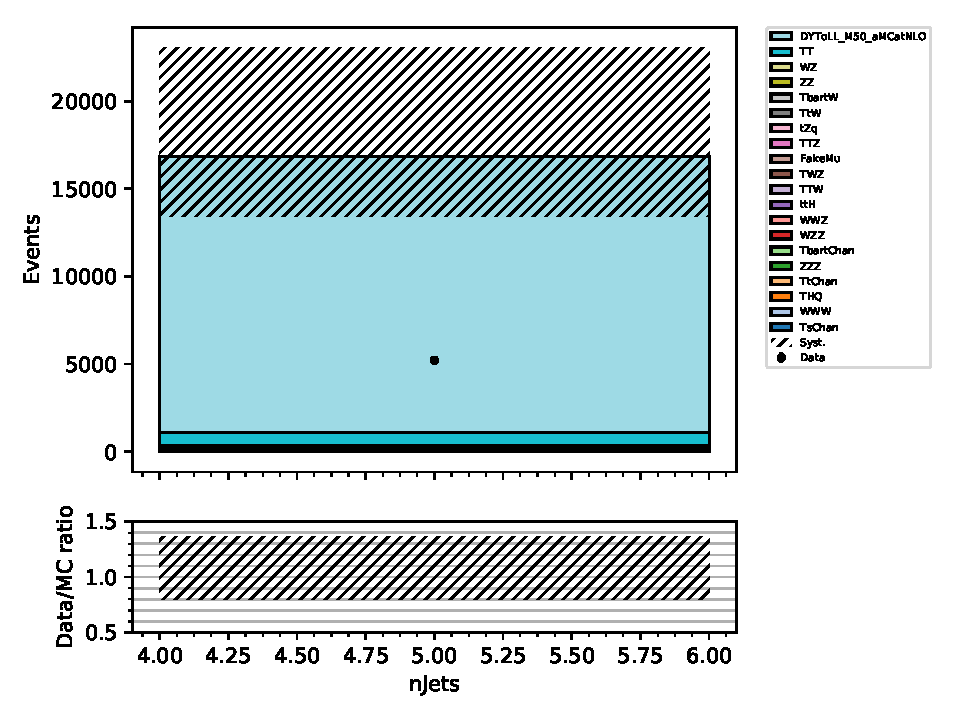
\includegraphics[width=0.47\textwidth]{figs/tzq-fullSelection-plots/plots_ee_zPlus/nJets.pdf}
\caption{
The distributions of the number of jets in the nominal Z+jets control region following the application of the full control region event selection and simulation corrections for the combination of both channels.
}
\label{fig:zPlusCR_nJets}
\end{figure}

\begin{figure}[tbp]
\centering
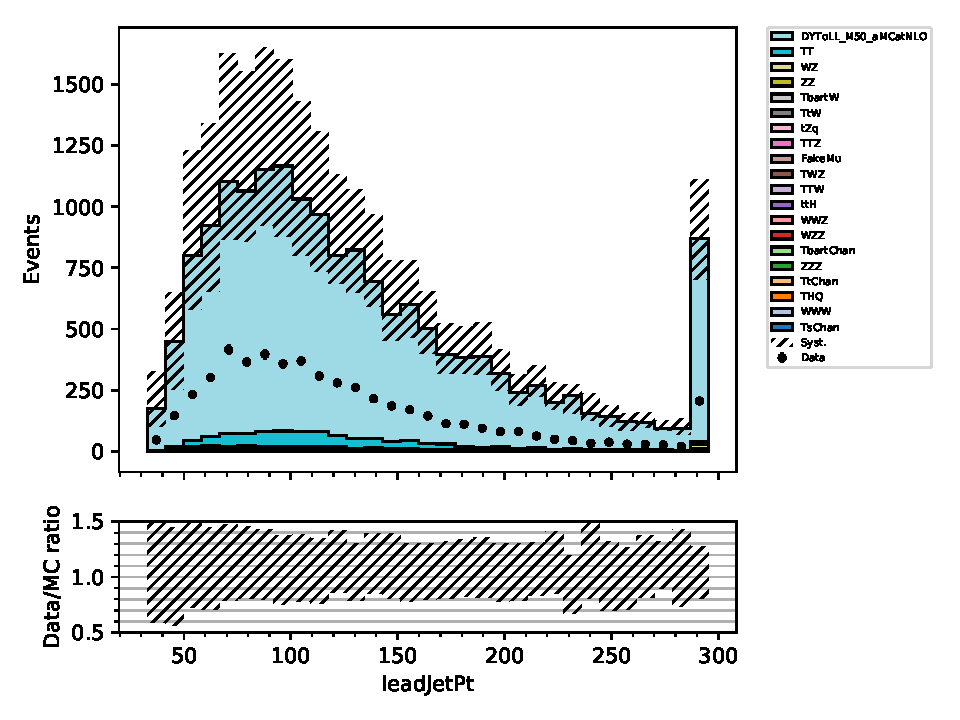
\includegraphics[width=0.47\textwidth]{figs/tzq-fullSelection-plots/plots_ee_zPlus/leadJetPt.pdf}
\caption{
The distributions of the leading jet \pt in the nominal Z+jets control region following the application of the full control region event selection and simulation corrections for the combination of both channels.
}
\label{fig:zPlusCR_leadJetPt}
\end{figure}

\begin{figure}[tbp]
\centering
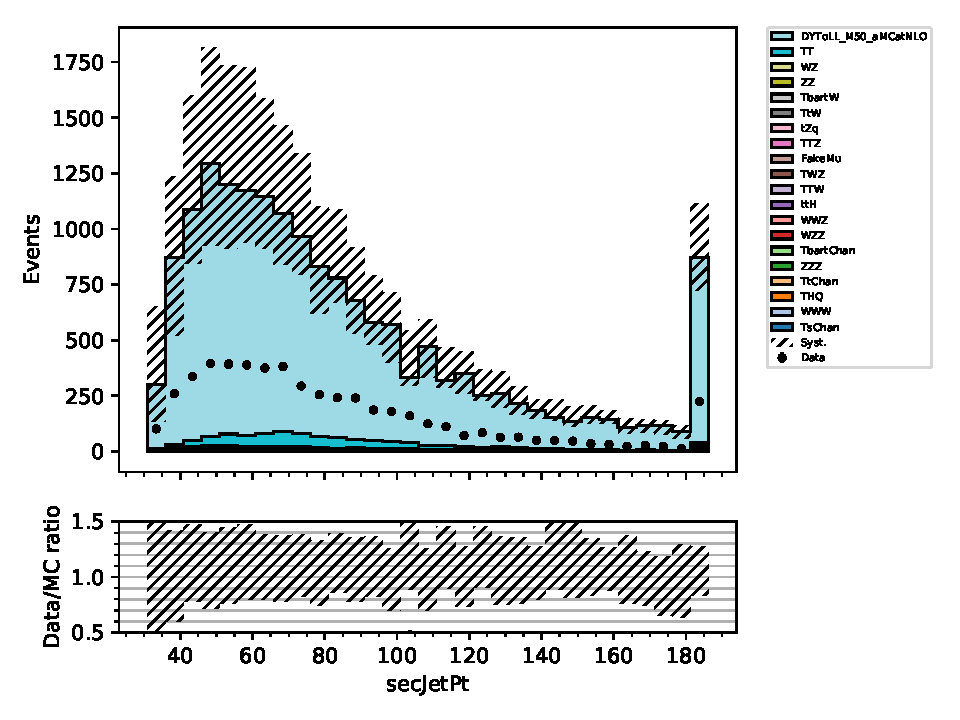
\includegraphics[width=0.47\textwidth]{figs/tzq-fullSelection-plots/plots_ee_zPlus/secJetPt.pdf}
\caption{
The distributions of the subleading jet \pt in the nominal Z+jets control region following the application of the full control region event selection and simulation corrections for the combination of both channels.
}
\label{fig:zPlusCR_secJetPt}
\end{figure}

\begin{figure}[tbp]
\centering
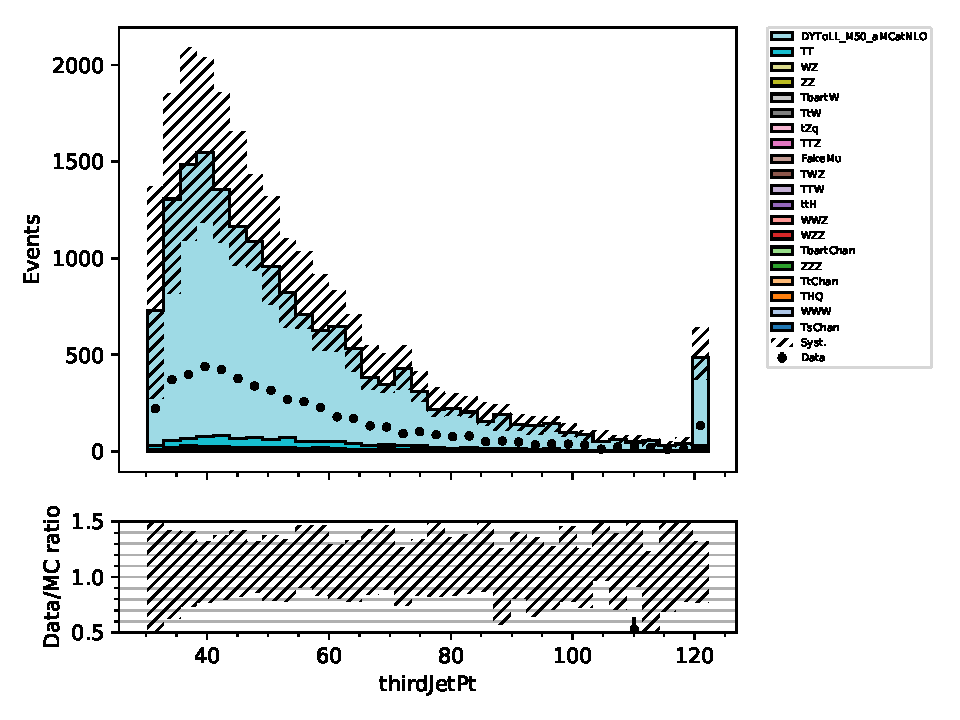
\includegraphics[width=0.47\textwidth]{figs/tzq-fullSelection-plots/plots_ee_zPlus/thirdJetPt.pdf}
\caption{
The distributions of the third jet \pt in the nominal Z+jets control region following the application of the full control region event selection and simulation corrections for the combination of both channels.
}
\label{fig:zPlusCR_thirdJetPt}
\end{figure}

\begin{figure}[tbp]
\centering
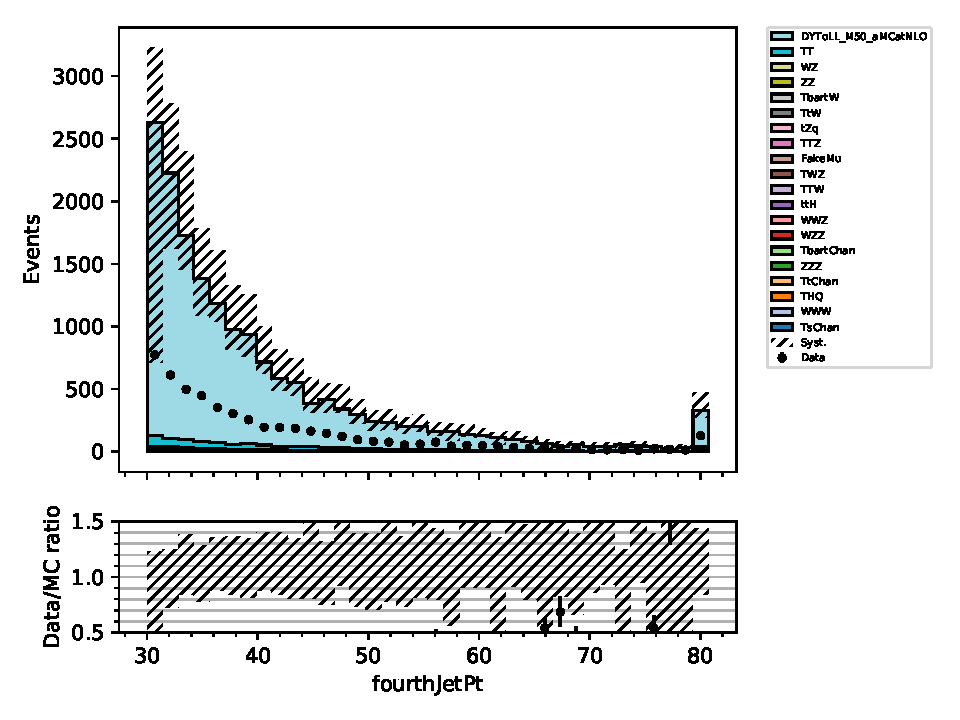
\includegraphics[width=0.47\textwidth]{figs/tzq-fullSelection-plots/plots_ee_zPlus/fourthJetPt.pdf}
\caption{
The distributions of the fourth jet \pt in the nominal Z+jets control region following the application of the full control region event selection and simulation corrections for the combination of both channels.
}
\label{fig:zPlusCR_fourthJetPt}
\end{figure}

Following observing this normalisation offset, a number of alternative Z+jets samples which were binned as a function of the Z boson's \pT and the number of jets produced by the hard process were also considered.
In contrast to the nominal Z boson mass binned samples, the alternative Z+jets samples generated by Madgraph and aMC@NLO were found to poorly describe the shapes of Z boson and jet distributions.
Consequently, these alternative samples were not considered as viable replacements of the Z boson mass binned Z+jets samples.

As having a NLO description of this large multi-jet background was highly desirable in light of the event selection requirements, it was decided to use nominal Z+jets control region to determine the correct normalisation of the aMC@NLO Z+jets samples.
This was achieved by simultaneously fitting this background in the control region at the same time as the signal region fit was performed.

\subsection{\ttbar Background}\label{subsec:ttbarEstimation}
The \ttbar enriched control region, as defined in Section~\ref{subsec:ttbarCR}, was designed to provide an orthogonal region which was topologically similar to the signal region.
This was done to validate whether or not the simulated \ttbar sample used accurately modelled the \ttbar process in the data, and if not, to be used to derive a data-driven estimate for \ttbar.

As good agreement was observed between data and MC simulation for both the overall normalisation and the shapes of individual variables, it was determined that a data-driven estimate of the \ttbar contribution was not necessary.

Examples of this good agreement can be seen in the distributions of the number of jets and b-jets in figure~\ref{fig:ttbarCR_nJets}, the \pT of the four leading jets in figure~\ref{fig:ttbarCR_jetPt}, and the \pT of each of the leptons and the invariant mass and \pT in figure~\ref{fig:ttbarCR_leptons}.

Table~\ref{tab:ttbarCR} shows that after these selection criteria and the required simulation corrections discussed in Section~\ref{sec:simCorrections} have been applied, the resulting control region has a 94.5\% purity and that half of the backgrounds are from tW single top production.
\begin{table}[htbp]
\topcaption {
The event yields, and the uncertainties associated with them, following the full event selection and simulation corrections for the \ttbar control region. The non-prompt lepton contribution is estimated using the methodology described in Section~\ref{sec:NPLs}.
}
\label{tab:ttbarCR}
  \centering
% This right-aligns numbers in column, but centers them under column title.
 \begin{tabular}{cc}
   \hline
   \textbf{MC process} & \textbf{$e\mu$}  \\
   \hline
	tZq\@: & 1.64$\pm$0.02  \\
	tWZ\@: & 11.62$\pm$0.07  \\
	tHq\@: & 1.15$\pm$0.27  \\
	ttW\@: & 50.09$\pm$0.30   \\
	ttZ\@: & 45.17$\pm$0.26   \\
	ttH\@: & 34.02$\pm$0.25  \\
	\ttbar: & 11832.4$\pm$60.3   \\
	tW\@: & 489.56$\pm$12.08   \\
	s-channel\@: &  0.0$\pm$0.0 \\
	t-channel\@: & 1.75$\pm$0.44 \\
	WW\@: & 11.36$\pm$1.39  \\
	WZ\@: & 3.87$\pm$0.29 \\
	ZZ\@: & 0.69$\pm$0.05 \\
	WWW\@: & 0.85$\pm$0.15     \\
	WWZ\@: & 0.43$\pm$0.12     \\
	WZZ\@: & 0.07$\pm$0.02     \\
	ZZZ\@: & 0.01$\pm$0.01     \\
	W + jets\@: & 23.39$\pm$16.54     \\
	Z + jets\@: & 19.64$\pm$5.07     \\
	\hline
%	NPLs\@: & 406.38$\pm$1.87     \\
	\hline
	Data\@: & 12498.0$\pm$111.79     \\
	\hline
	Total MC\@: & 12527.71$\pm$142.63     \\
   \hline
 \end{tabular}
\end{table}


\begin{figure}[tbp]
\centering
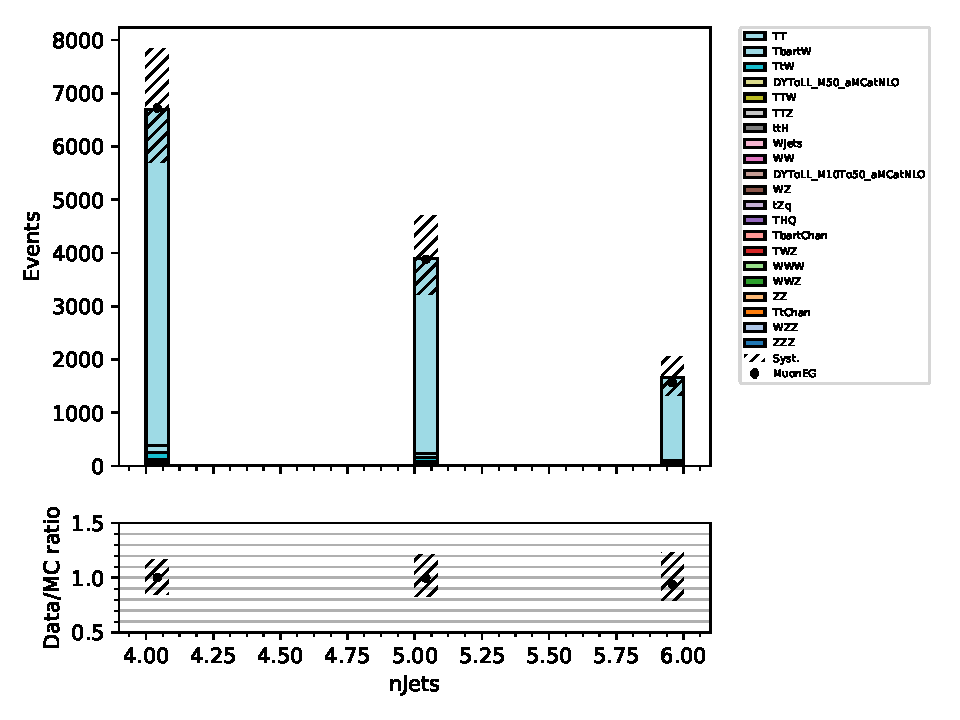
\includegraphics[width=0.47\textwidth]{figs/tzq-fullSelection-plots/plots_emu/nJets.pdf}
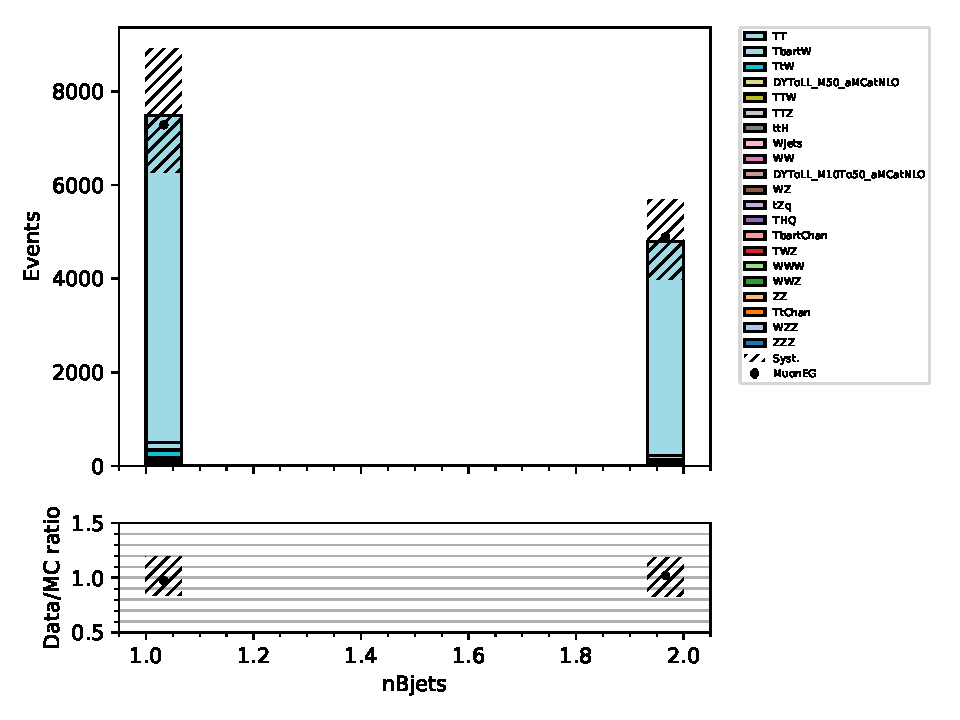
\includegraphics[width=0.47\textwidth]{figs/tzq-fullSelection-plots/plots_emu/nBjets.pdf}
\caption{
The distributions of the number of jets and the number b-tagged jets for the \ttbar control region following the application of the full control region event selection and simulation corrections.
}
\label{fig:ttbarCR_nJets}
\end{figure}

\begin{figure}[tbp]
\centering
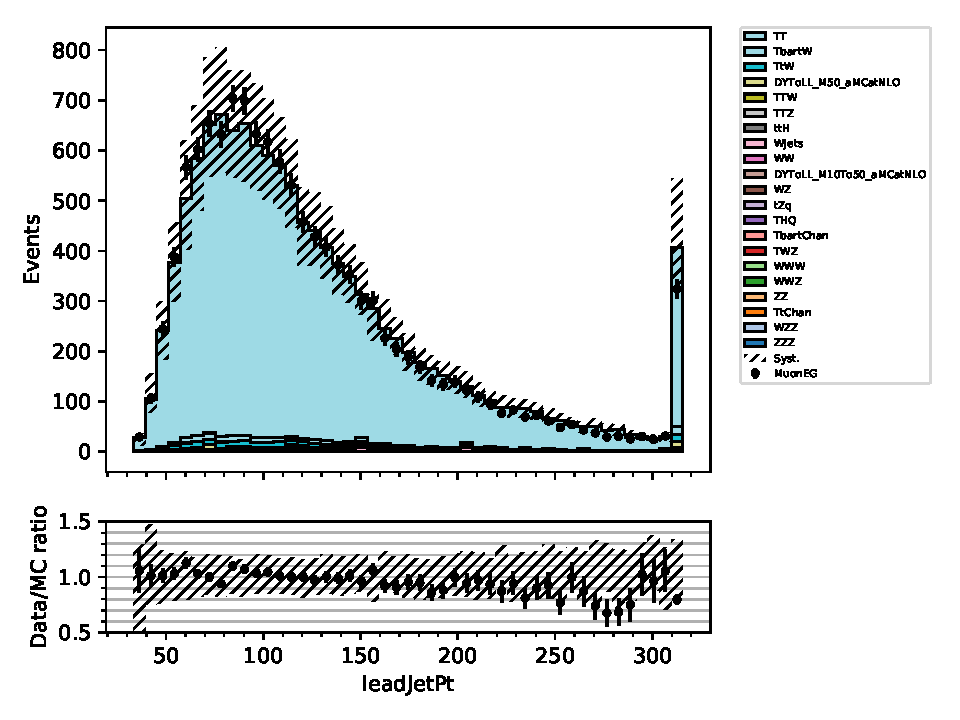
\includegraphics[width=0.47\textwidth]{figs/tzq-fullSelection-plots/plots_emu/leadJetPt.pdf}
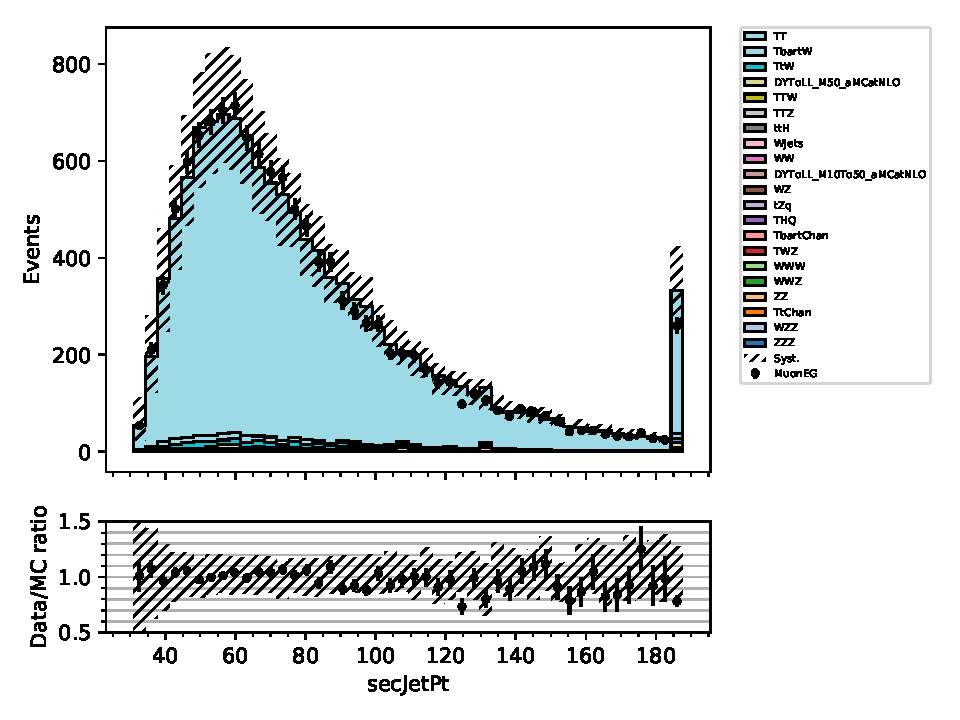
\includegraphics[width=0.47\textwidth]{figs/tzq-fullSelection-plots/plots_emu/secJetPt.pdf}
\\
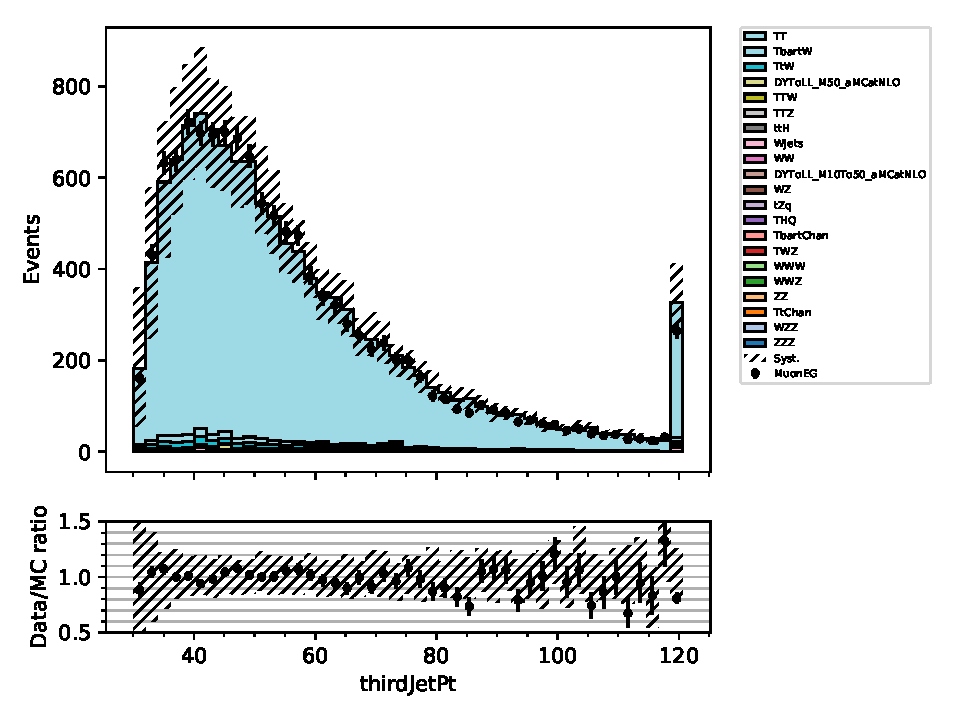
\includegraphics[width=0.47\textwidth]{figs/tzq-fullSelection-plots/plots_emu/thirdJetPt.pdf}
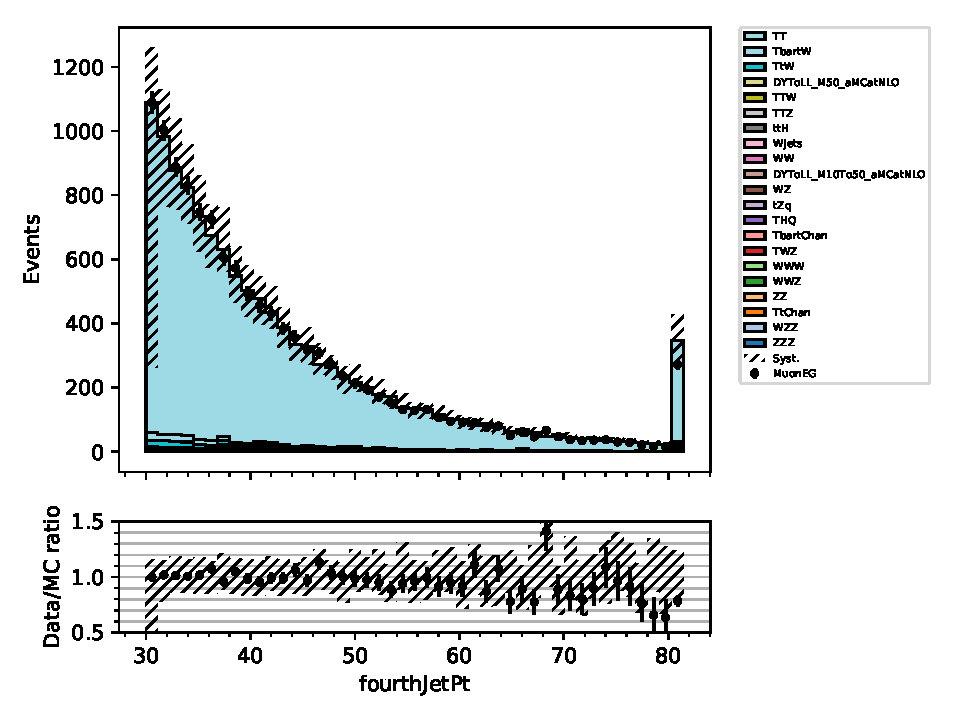
\includegraphics[width=0.47\textwidth]{figs/tzq-fullSelection-plots/plots_emu/fourthJetPt.pdf}
\caption{
The distribution of the \pt of the four leading jets for the \ttbar control region following the application of the full control region event selection and simulation corrections.
}
\label{fig:ttbarCR_jetPt}
\end{figure}

\begin{figure}[tbp]
\centering
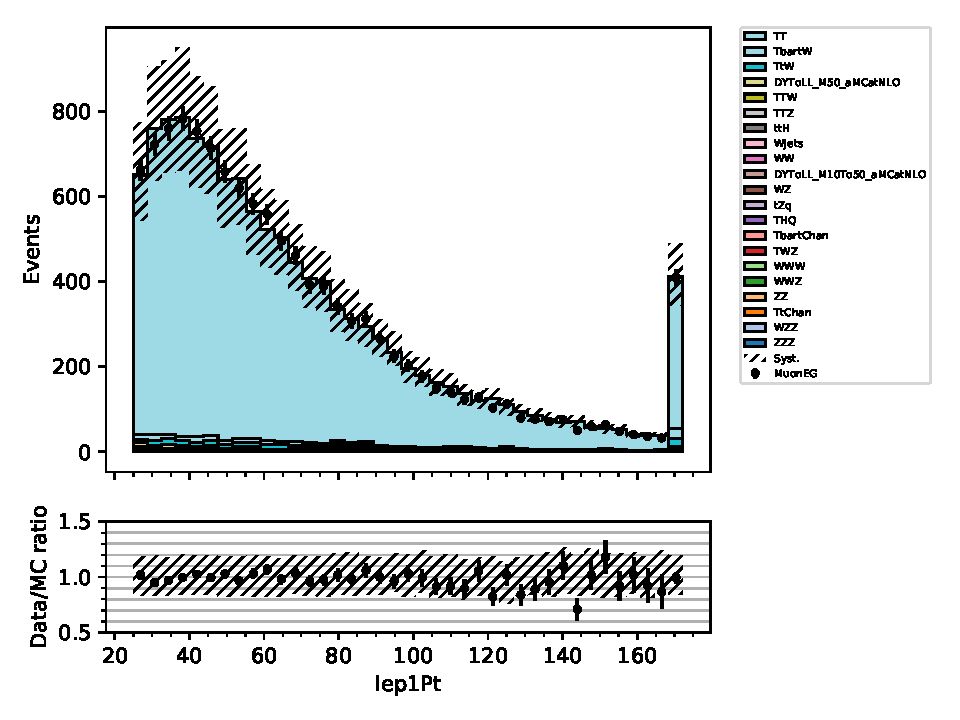
\includegraphics[width=0.47\textwidth]{figs/tzq-fullSelection-plots/plots_emu/lep1Pt.pdf}
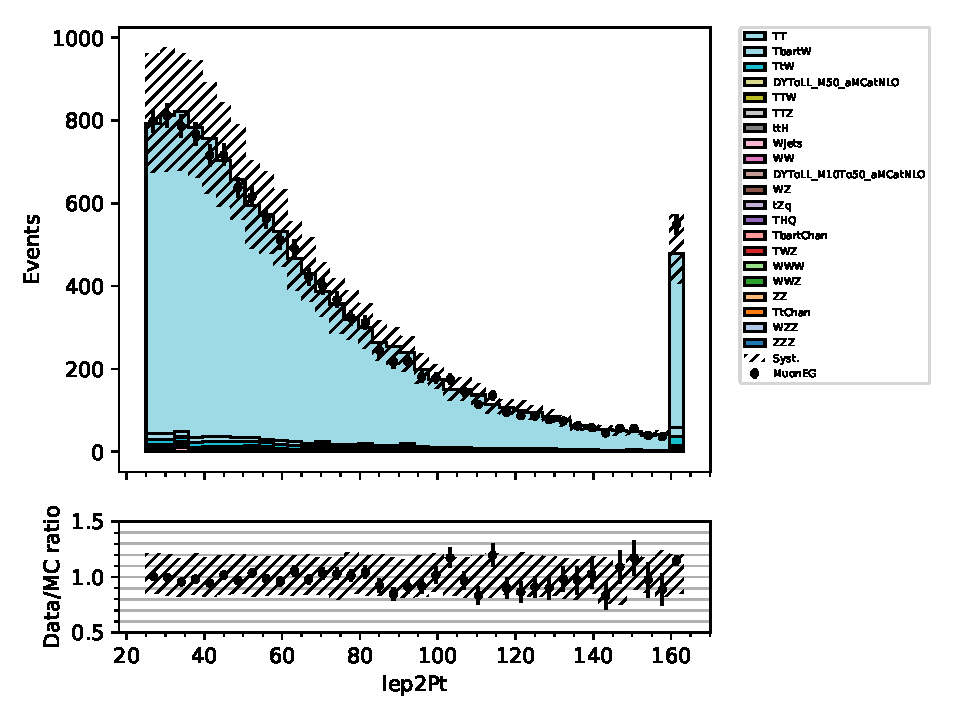
\includegraphics[width=0.47\textwidth]{figs/tzq-fullSelection-plots/plots_emu/lep2Pt.pdf}
\\
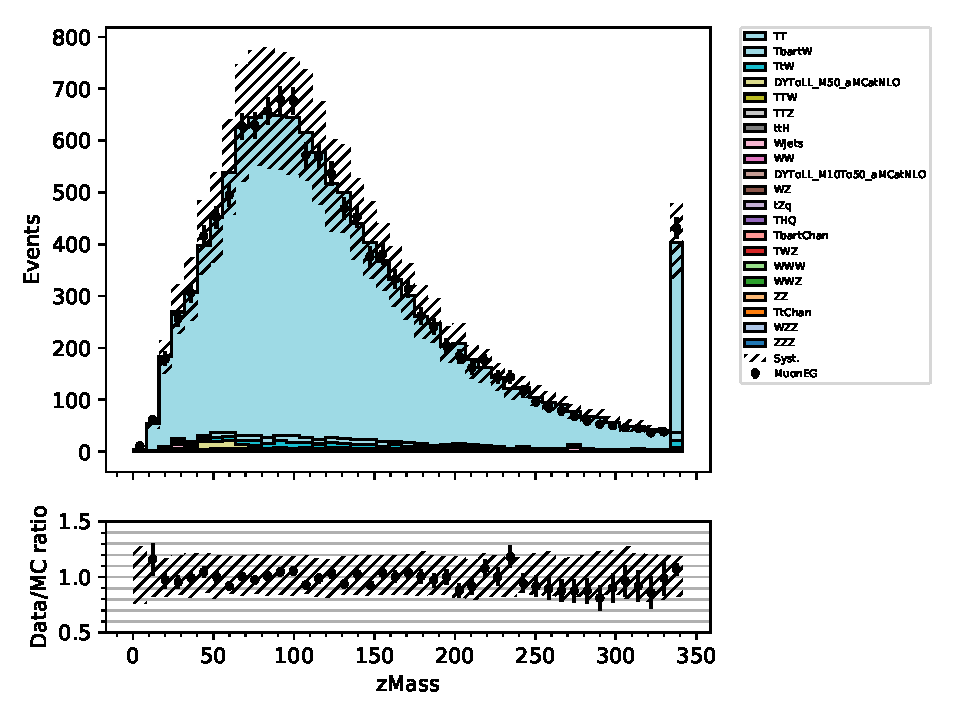
\includegraphics[width=0.47\textwidth]{figs/tzq-fullSelection-plots/plots_emu/zMass.pdf}
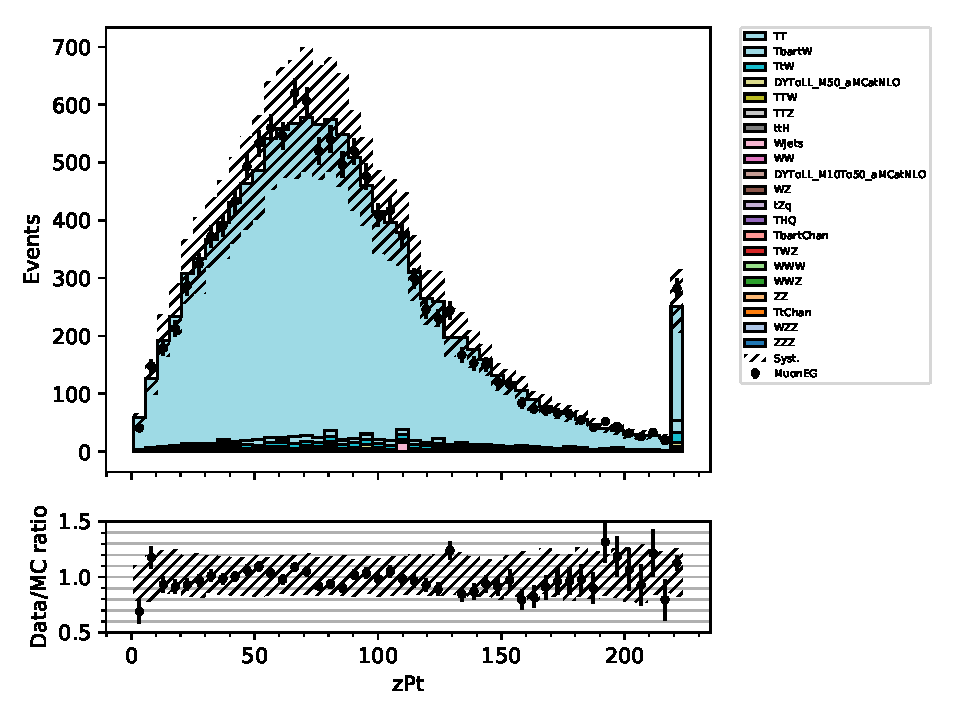
\includegraphics[width=0.47\textwidth]{figs/tzq-fullSelection-plots/plots_emu/zPt.pdf}
\caption{
The distribution of the selected electron and muon \pT and their combined invariant mass and \pt for the \ttbar control region following the application of the full control region event selection and simulation corrections.
}
\label{fig:ttbarCR_leptons}
\end{figure}


\section{Multivariate Analysis Techniques}\label{sec:mvas}
Multivariate Analysis (MVA) techniques are used to enhance the separation between signal and background processes which are difficult to discriminate between by applying individual selection criteria.

Therefore, a MVA technique was used to enhance the separation between the signal process from the background processes present following the application of the selection requirements described in Chapter~\ref{chapter:tzq-search}.
\emph{Boosted Decision Trees}~(BDTs) were chosen for this analysis as they were found to give superior performance compared to other MVA techniques and they are a widely used and supported technique with CMS existing expertise.

\subsection{Boosted Decision Trees}\label{subsec:bdt}
As illustrated in Figure~\ref{fig:decisionTree}, a decision tree is a series of sequential binary decisions (nodes) used to classify an event.
Each node compares a single input variable (\emph{feature}) against a threshold to determine which of the next two nodes it'll be sent to.
After a final decision
 are made on a single input variable (\emph{feature}), $x_{i}$, until a final decision is made at a terminating or \emph{leaf node} and the object is classified as either signal (S) or background (B).

\begin{figure}[htb]
\centering
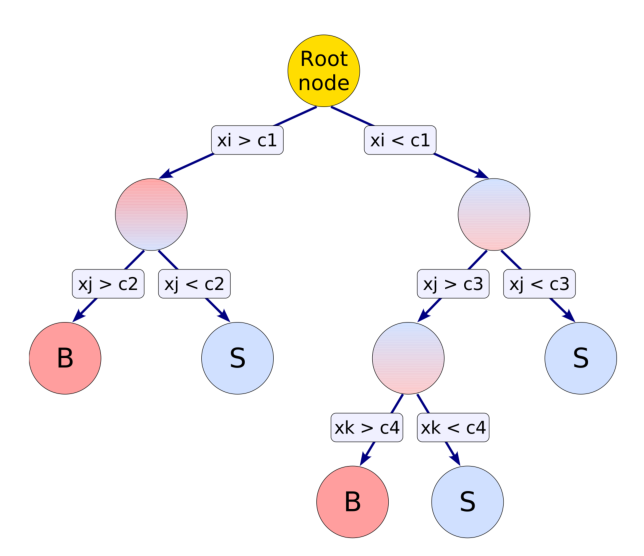
\includegraphics[width=0.97\textwidth]{figs/background-estimation/decisionTree.pdf}
\caption{A simple decision tree where repeated cuts a member of the set of variables $\textbf{x}$ are perfomed until a leaf node is reached and the object is classified as either signal (S) or background (B)~\cite{Hocker:2007ht}.
}
\label{fig:decisionTree}
\end{figure}

As the decision criterion for each node is dependent on the decisions of the preceding nodes, decision trees have the potential to obtain better separation between signal and background processes through individual cuts on isolated variables.
Without any prior knowledge of the system however, a single isolated tree is not expected to be an efficient classifier.
Despite this however, such a weak learner will still contain some knowledge about the underlying structure of the classification problem.

\emph{Boosting} aims to exploit this knowledge by using an ensemble of repeatedly trained weak learners to produce a more effective classifier.
Following each training iteration the dataset is reweighted based on the success of the previous classifiers in order to force the weak learners to attempt to classify objects that are harder to identify.
At the end of this process a weighted average (based) of all the weak learners are combined to produce a single strong learner.

\emph{Bagging} is a similar concept to boosting, but involves each weak learner being trained on a random subset of the training sample, such that every element has an equal probability of being sampled.

Therefore by extending boosting (or bagging) to decision trees, the resultant forest of \emph{Boosted Decision Trees} produces a classifier that is both much more effective and resilient to fluctuations in the training sample than one created by a single tree.

Typically the classifier produced by a BDT takes the form of a single discriminator whose response ranges between -1 to +1, denoting completely background-like and signal-like objects, respectively.

Two of the most common boosting algorithms used with decision trees are the Adaptive Boosting (\emph{AdaBoost})~\cite{Friedman:additivelogistic} and \emph{Gradient Boosting}~\cite{Friedman:greedyfunction,Friedman:GradientBoosting} algorithms.
Adaboost adjusts the weighting assigned to both  misclassified objects and the best performing weak learners after each iteration so that the best learners are trained to correctly identify the most difficult objects.
In contrast, gradient boosting uses gradient descent following each iteration to determine the residuals of the objects in order to focus on correctly classifying the objects with the largest residuals.

Despite their effectiveness however, BDTs are particularly sensitive to the effects of \emph{overtraining}.
This phenomena occurs when BDT is overly optimised on correctly classifying the training dataset and results in the poor classification of unseen data.
To minimise the impact of any potential overtraining, the signal and background process samples are split into training and testing samples, where the latter samples are used to check the validity of the BDT trained with the former.
A description of the training and testing method used to validate both the optimisation of the selection of the hyperparameters and whether or not they were overtrained is given in Section~\ref{subsec:hyperparameters}.


A number of studies were performed to determine the optimal settings for this analysis.
These included the evaluation of:

\begin{itemize}
\item a number of different boosting and bagging algorithms;
\item which simulated background processes should be included in the training processes;
\item whether or not multiple BDTs trained on separate backgrounds would be more effective than a single BDT;
\item how to determine which features possessed the greater discriminating power;
\item and which \emph{hyperparameters}, the set of options used to control BDT behaviour, and associated values gave the optimal classification performance.
\end{itemize}

It was determined that the \emph{eXtreme Gradient Boosting} (XGBoost) implementation of the Gradiant Boost algorithm for a single BDT trained on all the MC simulation samples gave the optimal performance for this search~\cite{xgboost}.

The methods used for selecting these features and the model hyperparameters are described in the following subsections.
Both the input features and model hyperparameters were chosen separately for $ee$ and $\mu\mu$ channels and all the simulated MC samples were considered.

\subsection{BDT Optimisation}
From the selected reconstructed physics objects, a large number of possible input variables or \emph{features} were constructed and considered as inputs for the BDT.
In order to determine the optimal set of features, recursive feature elimination was used to those that had the greatest discriminating power between signal and background.
This process iteratively removes the least important feature and re-trains the BDT until every feature has been ranked in order of their removal (\ie in increasing order of their discriminating power).
From this list, the features with the best discriminating power are selected for use in the BDT.

The features chosen by this process for the $ee$ and $\mu\mu$ channels are given in table~\ref{tab:selectedBdtVariables}.
Figure~\ref{fig:inputFeaturesDistributions} shows the distributions of the selected features in the signal and background samples.
Figure~\ref{fig:inputFeaturesDataSimAgreement} shows good agreement observed between simulation and data for the two channels for the features selected, demonstrating their reliability.
Table~\ref{tab:allBdtVariables}, in Appendix~\ref{app:bdt}, provides a list of all the features that were considered.

\begin{table}[htbp]
\topcaption {The name and descriptions of the variables chosen by recursive feature elimination to be used as input to the BDT to discriminate between potential tZq signal events and the dominant backgrounds.
}
\label{tab:selectedBdtVariables}
  \centering
% This increases column spacing.
\resizebox{\textwidth}{!}{
% This right-aligns numbers in column, but centers them under column title.
\begin{tabular}{cccc}
   \hline\
   \multirow{2}{*}{\textbf{Feature}} & \multirow{2}{*}{\textbf{Description}} & \multicolumn{2}{c}{\textbf{Discriminating Power}} \\
   & & \textbf{$ee$} & \textbf{$\mu\mu$} \\
   \hline
    bTagDisc & Leading b-tagged jet b-tag output discriminant & 0 & $4.529 \times 10^{-2}$ \\ 
    fourthJetPt & Fourth jet \pt & - & $3.391 \times 10^{-2}$ \\ 
    jetHt & ${\ensuremath{H_{\mathrm{T}}}}$ of all the jets in an event & - & $3.413 \times 10^{-2}$ \\ 
    jetMass & Total mass of every jet in an event & $1.467 \times 10^{-1}$  & $5.747 \times 10^{-2}$  \\
    jjDelR & $\Delta R$ between the leading jets & $5.778 \times 10^{-2}$  & $6.405 \times 10^{-2}$  \\ 
    leadJetEta & Leading jet $\eta$ & $2.222 \times 10^{-2}$ & $6.756\times 10^{-2}$  \\
    leadJetPt & Leading jet \pt & $0$ & $4.098 \times 10^{-2}$  \\ 
    zEta & Reconstructed Z boson $\eta$ & - & $6.129 \times 10^{-2}$ \\
    lepHt & ${\ensuremath{H_{\mathrm{T}}}}$ of the Z boson candidate's leptons & - & $5.325 \times 10^{-2}$ \\
    met & Missing transverse energy & $1.822 \times 10^{-1}$  & $7.587 \times 10^{-2}$  \\
    secJetPt & Second jet \pt & -  & $3.916 \times 10^{-2}$  \\
    thirdJetPt & Third jet \pt & $0$  & $3.613 \times 10^{-2}$  \\ 
    topMass & Reconstructed top quark mass & $1.067 \times 10^{-1}$  & $8.076 \times 10^{-2}$  \\
    totHtOverPt & Total ${\ensuremath{H_{\mathrm{T}}}}$ divided by total \pt & $1.200 \times 10^{-1}$  & $5.738 \times 10^{-2}$  \\
    wPairMass & Reconstructed W boson mass & -  & $4.894 \times 10^{-2}$  \\
    wQuark2Eta & Subleading W boson candidate jet $\eta$ & - & $4.342 \times 10^{-2}$ \\
    zMass & Reconstructed Z boson mass & $3.644 \times 10^{-1}$  & $7.085 \times 10^{-2}$  \\
    zTopDelR & $\Delta R$ between the Z boson and top quark candidates & - & $4.778 \times 10^{-2}$ \\
    zjminR & Minimum $\Delta R$ between the Z boson candidate and any jet & - & $4.178 \times 10^{-2}$ \\
   \hline
 \end{tabular}}
\end{table}

\begin{figure}[tbp]
\centering

\includegraphics[width=0.97\textwidth]{CMS-bw-logo.pdf}
\caption{
Distributions of the features chosen for use with the BDT for the signal and background samples.}
\label{fig:inputFeaturesDistributions}
\end{figure}

\begin{figure}[tbp]
\centering

\includegraphics[width=0.97\textwidth]{CMS-bw-logo.pdf}
\caption{
Distributions of the ... for the combination of the $ee$ and $\mu\mu$ channel}
\label{fig:inputFeaturesDataSimAgreement}
\end{figure}

Instead of tuning the choice hyperparmeters for optimal classification performance either by hand or a time and computationally expensive grid search, the optimal choice of hyperparmeters was evaluated using the \emph{Scikit-Optimize} library~\cite{scikit-optimise} to construct and evaluate a regression model based on a Gaussian process.
Table~\ref{tab:hyperparameters} lists the optimal hyperparameters for the $ee$ and $\mu\mu$ channels were that were determined by the \emph{Scikit-Optimize} regression model.

\begin{table}[htbp]
\topcaption {The optimal hyperparameters for the $ee$ and $\mu\mu$ channels for XGBoost that were found by \emph{Scikit-Optimize} and the maximum and minimum values that they can take.
}
\label{tab:hyperparameters}
  \centering
% This increases column spacing.
\resizebox{\textwidth}{!}{
% This right-aligns numbers in column, but centers them under column title.
\begin{tabular}{lccccc}
   \hline
   \textbf{Option} & \textbf{Min} & \textbf{Max} & \textbf{$ee$} & \textbf{$\mu\mu$}\\
   \hline
    gamma & $10^{-5}$ & 100 & 9.79 \\
    learning\_rate & $10^{-5}$ & 10 & $5.70 \times 10^{-2}$ \\
    max\_depth & 2 & 10 & 5 & 3\\
    min\_child\_weight & $10^{-5}$ & 100 & 30.6 & 3.40 \\
    n\_estimator & 25 & 7500 & 2338 & 6280 \\
    reg\_alpha & $10^{-5}$ & 1000 & $2.31 \times 10^{-3}$ & $1.33 \times 10^{-2}$ \\
    reg\_lambda & $10^{-5}$ & 1000 & 71.5 & $1.96 \times 10^{-4}$ \\
    subsample & 0.5 & 1 & 0.504 & 0.801 \\
   \hline
 \end{tabular}}
\end{table}

Following the optimisation of both the BDT features and the choice of hyperparameters for both channels independently, the optimal BDT is trained.
The BDT is then used to produce the distribution of the output discriminant for each of the data and simulation samples considered, including the dedicated simulation samples required to estimate the systematic uncertainties.
These output discriminant distributions are used to extract the signal strength and its statistical significance.


\section{Systematic Uncertainties}\label{sec:systematics}
%%% Intro
For any meaningful and robust measurement to be made in any physics analysis, it is vital that the sources of systematic uncertainties associated with it are both understood and controlled.
This is particularly important for this analysis as the low signal process production cross section compared to those of the backgrounds result in the scale of the statistical uncertainties being comparable to that of the systematic uncertainties of the measurement.

These sources of uncertainty originate from either experimental or theoretical uncertainties and influence the normalisation of the distributions considered and/or the shape of the distributions.
The statistical uncertainties arising from the size of the simulated samples available are also considered.

These uncertainties are treated as nuisance parameters in the signal extraction, which is described, along with the impact of the uncertainties on the result, in Section~\ref{sec:statisticalModel}.

\subsection{Experimental Uncertainties}
\subsubsection*{Jet Energy Corrections}
The CMS Jet Energy Corrections group provides the uncertainties associated with the JES and JER values they determine (discussed in Sections~\ref{subsubsec:JECs} and~\ref{subsec:jesjer})~\cite{Khachatryan:2016kdb}. 

The impact of the JES is evaluated by varying the JES values applied to all jets up and down by a standard deviation.
The uncertainty associated with the JER smearing is accounted for by varying the smearing factor up and down by the associated statistical uncertainty.

\subsubsection*{Missing Transverse Energy Uncertainties}
As missing transverse energy is calculated from the sum of the \pT of all PF objects in a given event along with the remaining unclustered energy deposits, the uncertainties associated with both have to be considered.

The impact of the uncertainties associated with both the JES and JER on the PF \MET are accounted for by propagating the JEC uncertainties through to the \MET and evaluating the impact they have.
As the unclustered energy remains uncorrected, the impact on the \MET uncertainty is evaluated by varying the contributions to the unclustered energy from each particle by their respective resolution.

\subsubsection*{Pileup Reweighting}
The uncertainty associated with the \PU reweighting (see Section~\ref{subsec:puSF}) is determined by varying the expected minimum bias cross section applied to the simulation simulation by $\pm X\%$.

\subsubsection*{Parton Density Functions}\label{subsec:pdfSysts}
%%Discussion of what PDFs are, is given in an earlier chapter 
As PDFs are derived from data measured by different experiments, the uncertainties associated with each measurement must be propagated to the momentum fractions and energies that have been assigned to partons of the incoming protons.

The impact of the PDF uncertainties are evaluated according to PDF4LHC recommendations~\cite{Butterworth:2015oua}, namely as the standard deviation of the weights of the nominal and the variations of the PDF set.

For almost all of the MC samples considered, this is achieved by considering the nonimal event weight and one hundred alternative PDF weights.

The single top tW-channel samples are the exception to this as at the time of their generation it was not possible to generate the required per-event weights.
In this case, the LHAPDF (Les Houches Accord Parton Distribution Function) library is used to access both the nominal PDF weight and the 100 eigenvalues from the NNPDF3.0 set needed to provide the required 200 alternative event weights.

\subsubsection*{b-tagging Uncertainties}
The uncertainties associated with the b-tagging scale factors described in Section~\ref{subsec:btagEff} are obtained by varying their value by $\pm 1\sigma$.

\subsubsection*{Non-prompt Lepton Contributions}
As the data-driven estimate of the NPL background contributions should have no dependence on either the lepton flavour or selection cuts.
Therefore the variation of the ratio of opposite-sign over same-sign events as a function of the lepton flavour and the cut level was considered to be well accounted for by a 30\% rate uncertainty.

\subsubsection*{Z+jets Background}
The uncertainty associated with the normalisation of the aMC@NLO Z+jets background sample is evaluated as part of the signal extraction process described in Section~\ref{sec:statisticalModel}.
This involves a simultaneous fit of the Z+jets background enriched control region and the signal region to measure the yields for both tZq and Z+jets processes.
As such, it incorporates the impact of the statistical uncertainty on the fit of the Z+jets control region as a nuisance parameter, which then controls the normalisation of the Z+jets contribution in the final signal region fit.

\subsubsection*{Luminosity Uncertainties}
%CMS uses the pixel detector, DTs, HF, the Fast Beam Conditions Monitor and Pixel Luminosity Telescope to monitor and measure the instantaneous and integrated luminosity.
%During Run 2, the primary offline luminosity measurements made by the CMS Luminosity Group used the pixel detector using the Pixel Cluster Counting (PCC) method due its stability over time for up an average \PU of 150 and the high precision results obtained with it during Run I.
%The PCC algorithm is able to achieve such a precision by measuring the instantaneous luminosity through the number of pixels present. 
%This is possible as the probability of pixel hit belonging to multiple tracks is very small due to the very low occupancy of the detector, inferring that the number of pixel hits are linearly proportional to the number of interactions during a bunch crossing~\cite{CMS:2017_lumi}.

%Van der Meer (VdM) scans during dedicated LHC runs were used to calibrate the absolute luminosity scale calibrations of the detectors~\cite{vanderMeer:1968zz}

%%%%


The overall uncertainty in the integrated luminosity collected by CMS in 2016 was estimated to be 2.5\%~\cite{CMS:2017_lumi}.

%The MC events produced are weighted by a scale factor in order to correctly normalise them with respect to the data they are compared against.
%This normalisation scale factor is given by:
%\begin{equation}
%SF_{dataset} = \frac{\pazocal{L} \sigma}{N_{MC}^{Events}}
%\end{equation}
%where $\pazocal{L}$ is the amount of total integrated luminosity considered in the data used, $\sigma$ the cross section of the MC sample considered and $N_{MC}^{Events}$ is number of simulated events considered for the process.

\subsubsection*{Lepton Efficiencies}
The uncertainties associated with the lepton identification, isolation and reconstruction efficiency scale factors discussed in Section~\ref{subsec:leptonRecoSFs} are varied by $\pm 1 \sigma$.

Several systematic studies were performed to estimate the systematic uncertainty associated with the trigger scale factors.
These studies were the comparison of the trigger efficiencies \ttbar and Z+jets processes in simulation and the strength of the correlation of the \MET trigger selection to the lepton triggers used in the analysis.

As shown in table~\ref{tab:zPlusTriggerSFs} the differences in the triggers efficiencies observed in all channels are so small that they are covered by the statistical uncertainties.

\begin{table}[htbp]
\topcaption {
The trigger efficiencies for the lepton selection criteria for \ttbar and Z+jets in simulation.
The uncertainties given only include the statistical uncertainty associated with each value. 
}\label{tab:zPlusTriggerSFs}
  \centering
%  \resizebox{\textwidth}{!}{
% This right-aligns numbers in column, but centers them under column title.
 \begin{tabular}{llc}
   \hline
   \textbf{Channel} & \textbf{MC Sample} & \textbf{$\epsilon _{MC}$} \\
   \hline   
   \multirow{2}{*}{$ee$} & \ttbar & 0.98823 $\pm$ 0.00086 \\
   & Z+jets & 0.98849 $\pm$ 0.00106 \\
   \multirow{2}{*}{$\mu\mu$} & \ttbar & 0.99192 $\pm$ 0.00074 \\
   & Z+jets & 0.99258 $\pm$ 0.00083 \\
   \multirow{2}{*}{$e \mu$} \ttbar & 0.99148 $\pm$ 0.00722 \\
   & Z+jets & 0.98838 $\pm$ 0.01183 \\
   \hline
 \end{tabular}%}
\end{table}

In order to evaluate the independence of the \MET and lepton triggers used, the efficiency of each set of triggers is first considered individually.
If both sets triggers are independent, then the efficiency of fulfilling both trigger selections can be expressed as:

\begin{equation}
\frac{\epsilon_{X + lepton triggers}}{\epsilon_{X triggers} \times \epsilon_{lepton triggers}} = \alpha
\label{eq:triggerCorrelation}
\end{equation}

If the \MET and lepton trigger selection requirements are uncorrelated, then the ratio ($\alpha$) of the left and right hand sides of equation~\ref{eq:triggerCorrelation} will be 1.
Table~\ref{tab:triggerCorrelation} shows that for the all channels, $\alpha$ only exhibits small differences from unity, indicating negligible correlation between the triggers used.

\begin{table}[htbp]
\topcaption {
The values of $\alpha$, expressing the strength of correlation between the lepton and cross triggers used to determine the trigger scale factors, for each channel.
}\label{tab:triggerCorrelation}
  \centering
%  \resizebox{\textwidth}{!}{
% This right-aligns numbers in column, but centers them under column title.
 \begin{tabular}{cc}
   \hline
   \textbf{Channel} & \textbf{$\alpha$}   \\
   \hline   
   $ee$ & 0.99890 \\
   $\mu\mu$ & 1.00151  \\
   $e \mu$ & 0.98883  \\
   \hline
 \end{tabular}%}
\end{table}

%The impact on the scale factors of applying the analysis selection cuts following the dilepton selection criteria, and the minimum Z boson mass criteria used for the trigger efficiencies, was found to be ...
%
%\editComment{Update table with trigger efficiencies post selection cuts following revised trigger SFs}
%\begin{table}[htbp]
%\topcaption {
%Comparison of the trigger scale factors following the application of each of the event selection criteria.
%}\label{tab:eventSelectionImpactTriggerSF}
%  \centering
%  \resizebox{\textwidth}{!}{
%% This right-aligns numbers in column, but centers them under column title.
% \begin{tabular}{lccc}
%   \hline
%   \textbf{Selection criteria} & \textbf{$ee$} & \textbf{$\mu\mu$} & \textbf{$e \mu$} \\
%   \hline   
%   Dilepton & 0.98715 $\pm$ 0.00063 & 0.99318 $\pm$ 0.00015 & 0.99148 $\pm$ 0.00722 \\
%   4-6 jets  & 1.0 & 1.0 & 1.0 \\
%   1-2 b-jets & 1.0 & 1.0 & 1.0 \\
%   \hline
% \end{tabular}}
%\end{table}

%-----------------------------------------------------------
%Double Electron data efficiency: 0.14295 +/- -0.00030/0.00030
%Double Electron MC efficiency: 0.35126 +/- -0.00076/0.00076
%Double Electron trigger SF: 0.40696 +/- 0.00003
%-----------------------------------------------------------
%Double Muon data efficiency: 0.32028 +/- -0.00039/0.00039
%Double Muon MC efficiency: 0.41928 +/- -0.00078/0.00079
%Double Muon trigger SF: 0.76388 +/- 0.00049
%-----------------------------------------------------------
%MuonEG data efficiency: 0.20692 +/- -0.00059/0.00059
%MuonEG MC efficiency: 0.40262 +/- -0.00108 / 0.00108
%MuonEG trigger SF: 0.51393 +/- 0.00009
%-----------------------------------------------------------
%alpha for DoubleEG/DoubleMuon/MuonEG Triggers: 0.84805/1.04366/0.90554
%-----------------------------------------------------------
%-----------------------------------------------------------
%

Given the statistical uncertainties involved and the results of the studies briefly described above, it was determined that associating a systematic uncertainty of 1.0\%, 1.0\% and 2\% for the triggers used for the $ee$, $\mu\mu$, and $e \mu$ channels would be sufficient.

\subsection{Theoretical Uncertainties}\label{sec:theorySysts}
\subsubsection{Factorisation and renormalisation scales}
In order to consider the impact of the uncertainty associated with the choice of factorisation ($\mu_{F}$) and renormalisation scales ($\mu_{R}$) used in the ME and PS step of the generator, they are varied up and down by factors of 2 and 0.5, respectively.

%\editComment{WHAT IS Q2?}
%ISR : q^2 =  muR^2 = z(1-z)q^2; q^2 = -p^2
%FSR q^2 =  muR^2 = z(1-z)q^2; q^2 = p^2-m_0^2


Events weights are produced for the variation of $\mu_{F}$ and $\mu_{R}$ for the ME step where both scales are varied simultaneously in order to evaluate the impact of the $\mu_{f}$ and $\mu_{s}$ uncertainties.

In contrast to the ME level, the impact of the PS shower scale uncertainties was evaluated through the use of dedicated samples for certain processes.
In these samples the $\mu_{F}$ and $\mu_{R}$ 
These centrally produced samples are listed in Table~\ref{tab:theorySampleList} as the ``scale up'' and ``scale down'' samples. 
As mentioned above in Section~\ref{subsec:pdfSysts}, it was not possible for the single top tW-channel MC samples to be produced with per-event weights to account for the matrix element factorisation and renormalisation scales.
To account for this, the ``scale up'' and ``scale down'' samples listed in Table~\ref{tab:theorySampleList} for tW production also include the impact of varying $\mu_{F}$ and $\mu_{R}$ for the ME as well as the PS.
In the case of \ttbar however, the variations in the initial-state radiation (ISR) and final-state radiation (FSR) are considered separately.
The dedicated samples for these variations are listed in able~\ref{tab:theorySampleList} as the ``isr/fsr up'' and ``isr/fsr down'' samples for \ttbar production.

\subsubsection{Parton Shower Matching Thresholds}
As discussed in Section~\ref{subsec:eventGenerators}, all of the MC samples considered use model the hard scattering process through a dedicated Matrix Element generator, with PYTHIA 8 being used to perform the subsequent PS and hadronisation.

Dedicated samples evaluate the impact of the uncertainty associated with the choice of the energy threshold used for matching for the \ttbar and single top t-channel backgrounds generated with POWHEG, listed in table~\ref{tab:theorySampleList}.
For these samples, the model's matching threshold parameter is varied up and down by one standard deviation, effectively 

The uncertainty associated with the choice of the matching threshold for  quark samplse used is evaluated using dedicated matching samples where the matching threshold energy is varied up and down by one standard deviation~\cite{CMS:2016kle}.

\subsection{Pre-Fit Impact of the Systematic Uncertainties}\label{sec:uncertainitiesPreFitImpact}
The impact of the each of the systematics on the event yield (in percentage) of the simulated processes is shown in Table~\ref{tab:systImpact}.
These rates, whilst giving an overview of which systematics are the most important, do not show how the shape of the fitted variable, the BDT discriminant, is influenced by each uncertainty.

\begin{table}[!htbp]
\topcaption{Rate impact of systematics on MC templates}\label{tab:systImpact}
\begin{center}
\linespread{2}
\resizebox{\textwidth}{!}{\begin{tabular}{lcccccc}
\hline
Systematic      &  tZq                  & DY                   & \ttbar                  & \ttV         & VV &  Other \\
($ee$ / $\mu\mu$) & (\%)  & (\%)  & (\%)  & (\%)  & (\%)  &  (\%)   \\
\hline
Statistical &  $_{-0.24\%}^{+0.24\%}$ /  $_{-0.17\%}^{+0.17\%}$   & $_{-2.03\%}^{+2.03\%}$ / $_{-1.49\%}^{+1.49\%}$  & $_{-1.43\%}^{+1.43\%}$ / $_{-1.04\%}^{+1.04\%}$ & $_{-0.59\%}^{+0.59\%}$ / $_{-0.47\%}^{+0.47\%}$  \\
\hline
Lepton Eff.     &  $_{-5.41\%}^{+5.42\%}$ /  $_{-0.77\%}^{+4.87\%}$   & $_{-4.72\%}^{+4.07\%}$ / $_{-0.32\%}^{+6.37\%}$  & $_{-5.08\%}^{+4.41\%}$ / $_{-0.55\%}^{+5.54\%}$ & $_{-4.72\%}^{+4.85\%}$ / $_{-4.47\%}^{+5.97\%}$  \\
JES             &  $_{-0.17\%}^{+0.08\%}$ /  $_{-0.14\%}^{+0.14\%}$   & $_{-0.55\%}^{+0.29\%}$ / $_{-0.17\%}^{+0.13\%}$  & $_{-1.30\%}^{+0.02\%}$ / $_{-0.20\%}^{+0.20\%}$  & $_{-0.0.01\%}^{+0.11\%}$ / $_{-0.14\%}^{+0.18\%}$  \\
JER             &  $_{-5.27\%}^{+\%}$ /  $_{-6.11\%}^{+5.39\%}$   & $_{-11.81\%}^{+16.54\%}$ / $_{-14.18\%}^{+16.71\%}$  & $_{-7.98\%}^{+7.84\%}$ / $_{-6.13\%}^{+8.24\%}$  & $_{--1.96\%}^{+2.11\%}$ / $_{-1.62\%}^{+1.82\%}$  \\
Pileup             &  $_{-0.42\%}^{+0.43\%}$ /  $_{-0.17\%}^{+0.43\%}$   & $_{-2.35\%}^{+2.26\%}$ / $_{-2.57\%}^{+1.75\%}$  & $_{-1.52\%}^{+0.52\%}$ / $_{-0.09\%}^{+1.35\%}$  & $_{-0.86\%}^{+0.38\%}$ / $_{-0.15\%}^{+0.26\%}$  \\
PDF             &  $_{-9.98\%}^{+13.22\%}$ /  $_{-9.24\%}^{+11.94\%}$   & $_{-1.56\%}^{+1.73\%}$ / $_{-2.95\%}^{+2.16\%}$  & $_{-2.99\%}^{+1.85\%}$ / $_{-2.95\%}^{+2.16\%}$  & $_{-8.56\%}^{+9.95\%}$ / $_{-8.51\%}^{+9.40\%}$  \\
bTag             &  $_{-2.78\%}^{+3.38\%}$ /  $_{-3.38\%}^{+2.99\%}$   & $_{-5.30\%}^{+5.11\%}$ / $_{-5.02\%}^{+5.12\%}$  & $_{-2.89\%}^{+3.02\%}$ / $_{-3.12\%}^{+3.77\%}$  & $_{-3.43\%}^{+3.25\%}$ / $_{-3.24\%}^{+3.00\%}$  \\
ME             &  $_{-2.82\%}^{+1.36\%}$ /  $_{-3.06\%}^{+1.33\%}$   & $_{-15.00\%}^{+2.92\%}$ / $_{-14.64\%}^{+2.05\%}$  & $_{-11.38\%}^{-1.38\%}$ / $_{-11.40\%}^{+0.0\%}$  & $_{-5.01\%}^{+1.37\%}$ / $_{-5.07\%}^{+1.8\%}$  \\
PS             &  $_{-2.82\%}^{+1.36\%}$ /  $_{-3.06\%}^{+1.33\%}$   & $-$  & $_{-11.38\%}^{-1.38\%}$ / $_{-11.40\%}^{+0.0\%}$  & $_{-5.01\%}^{+1.37\%}$ / $_{-5.07\%}^{+1.8\%}$  \\
ME-PS Matching             & $-$   & $-$  & $_{-11.38\%}^{-1.38\%}$ / $_{-11.40\%}^{+0.0\%}$  & $_{-5.01\%}^{+1.37\%}$ / $_{-5.07\%}^{+1.8\%}$  \\
Luminosity             &  $_{-2.5\%}^{+2.5\%}$ /  $_{-2.5\%}^{+2.5\%}$    & $_{-2.5\%}^{+2.5\%}$  / $_{-2.5\%}^{+2.5\%}$   & $_{-2.5\%}^{+2.5\%}$  / $_{-2.5\%}^{+2.5\%}$   & $_{-2.5\%}^{+2.5\%}$  / $_{-2.5\%}^{+2.5\%}$   \\    
\hline
\end{tabular}
}
\end{center}
\end{table}
